% Do not add black pages at the end of a page
% From https://stackoverflow.com/a/1359496
\documentclass[oneside]{book}

% Change the font to Times.
% From https://stackoverflow.com/a/880794
\usepackage{times}

% Use slimmer margings
\usepackage[a4paper, total={7in, 10in}]{geometry}

% Show [number] [chapter title]
% (that is, without a newline after the chapter number) 
% From https://latex.org/forum/viewtopic.php?t=11650
\usepackage{titlesec}
\titleformat{\chapter}% reformat chapter headings
    [hang]% like section, with number on same line
    {\Huge\bfseries}% formatting applied to whole
    {\thechapter}% Chapter number
    {0.5em}% space between # and title
    {}% formatting applied just to title

% Remove vertical space in TOC between all chapters
% From https://tex.stackexchange.com/questions/235592/remove-vertical-space-between-several-chapters-in-toc
\usepackage{tocloft}
\setlength{\cftbeforechapskip}{0cm}

% Just try to parse, do not ask for input
\nonstopmode

% Bibliography
% For Vancounter style:
\usepackage[numbers]{natbib}
% For regular style:
% \usepackage{natbib}

% Just to have them already
% \begin{sloppypar}
% \end{sloppypar}



%\bibpunct{(}{)}{;}{a}{}{;}

% Use 'It was found that A is B (Name 1234)' style
%\setcitestyle{authoryear,open={},close={}}

% Affiliations
\title{
  Music
}
\author{Richèl J.C. Bilderbeek}


% Use double spacing
%\usepackage{setspace}
%\doublespacing

\usepackage{listings}
\usepackage{hyperref}
\usepackage{todonotes}
\usepackage{verbatim}
\usepackage{pgf}
\usepackage{bm}
\usepackage{multirow}
\usepackage{amsfonts}
\usepackage{array}
\usepackage{booktabs}
\newcolumntype{C}[1]{>{\centering\arraybackslash}p{#1}}
\newcolumntype{L}[1]{>{\raggedright\arraybackslash}p{#1}}
\usepackage{longtable}

% TikZ
\usepackage{tikz}
\usepackage{tkz-graph}
\usetikzlibrary{arrows,automata}

% sidewaysfigure
\usepackage{rotating}

% Style of listings
% From http://r.789695.n4.nabble.com/
%   How-to-nicely-display-R-code-with-the-LaTeX-package-listings-tp4648110.html
\usepackage{fancyvrb} 
\definecolor{codegreen}{rgb}{0,0.6,0}
\definecolor{codegray}{rgb}{0.5,0.5,0.5}
\definecolor{codepurple}{rgb}{0.58,0,0.82}
\definecolor{backcolor}{rgb}{0.95,0.95,0.92}
\lstdefinestyle{mystyle}{
  language={C++},% set programming language
  basicstyle=\ttfamily\small,% basic font style
  frame=single,
  commentstyle=\color{gray},% comment style
  numberstyle=\scriptsize,% use small line numbers
  numbersep=10pt,% space between line numbers and code
  tabsize=2,% sizes of tabs
  showstringspaces=false,
  captionpos=b,% positioning of the caption below
  breaklines=true,% automatic line breaking
%  escapeinside={(*}{*)},% escaping to LaTeX, don't: just keep those listings verbatim
  fancyvrb=true,% verbatim code is typset by listings
  extendedchars=false,% prohibit extended chars (chars of codes 128--255)
  deletekeywords={c}% remove keywords 
}
\lstset{style=mystyle}

% Subfigures
\usepackage{subcaption}

\begin{document}

% \maketitle

\tableofcontents

%%%%%%%%%%%%%%%%%%%%%%%%%%%%%%%%%%%%%%%%%%%%%%%%%%%%%%%%%%%%%%%%%%%%%%%%%%%%%%%%
\chapter{Maanliedje}
%%%%%%%%%%%%%%%%%%%%%%%%%%%%%%%%%%%%%%%%%%%%%%%%%%%%%%%%%%%%%%%%%%%%%%%%%%%%%%%%

%\lstinputlisting[
%  caption = Maanliedje,
%  label = lst:01_maanliedje
%]{../songs/01_maanliedje.txt}

\begin{figure}[!htbp]
  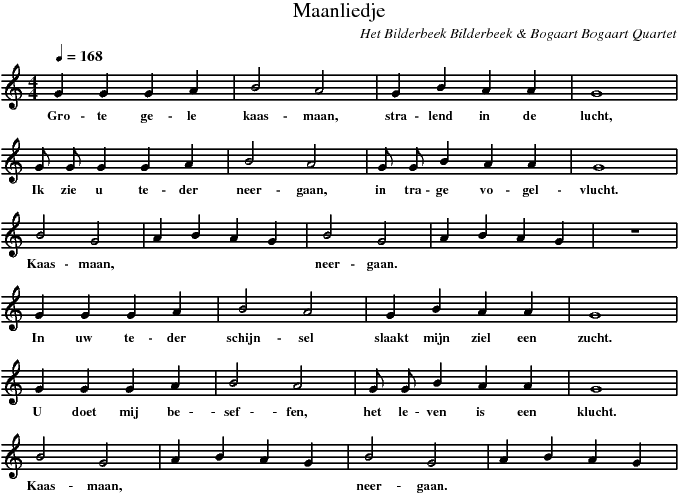
\includegraphics[width=\textwidth,height=\textheight,keepaspectratio]{../songs/01_maanliedje.png}
  \caption{Maanliedje}
  \label{fig:01_maanliedje}
\end{figure}


%%%%%%%%%%%%%%%%%%%%%%%%%%%%%%%%%%%%%%%%%%%%%%%%%%%%%%%%%%%%%%%%%%%%%%%%%%%%%%%%
\section{Grote gele sinaasappel}
%%%%%%%%%%%%%%%%%%%%%%%%%%%%%%%%%%%%%%%%%%%%%%%%%%%%%%%%%%%%%%%%%%%%%%%%%%%%%%%%

\lstinputlisting[
  caption = Grote gele sinaasappel,
  label = lst:02_grote_gele_sinaasappel
]{../songs/02_grote_gele_sinaasappel.txt}

\begin{figure}[!htbp]
  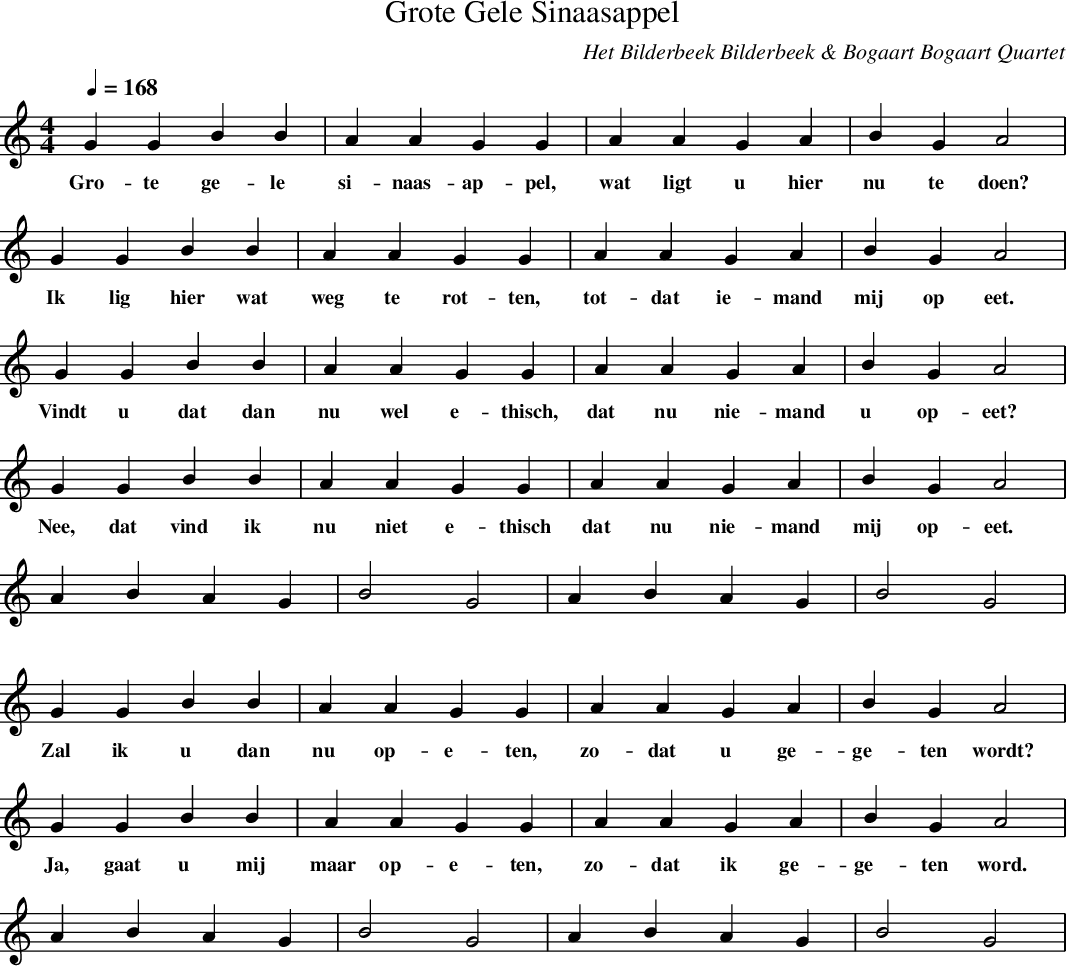
\includegraphics[width=\textwidth,height=\textheight,keepaspectratio]{../songs/02_grote_gele_sinaasappel.png}
  \caption{Grote gele sinaasappel}
  \label{fig:02_grote_gele_sinaasappel}
\end{figure}

%%%%%%%%%%%%%%%%%%%%%%%%%%%%%%%%%%%%%%%%%%%%%%%%%%%%%%%%%%%%%%%%%%%%%%%%%%%%%%%%
\chapter{Ode Aan Masculiniteit}
%%%%%%%%%%%%%%%%%%%%%%%%%%%%%%%%%%%%%%%%%%%%%%%%%%%%%%%%%%%%%%%%%%%%%%%%%%%%%%%%

%\lstinputlisting[
%  caption = Ode Aan Masculiniteit,
%  label = lst:03_ode_aan_masculiniteit
%]{../songs/03_ode_aan_masculiniteit.txt}

\begin{figure}[!htbp]
  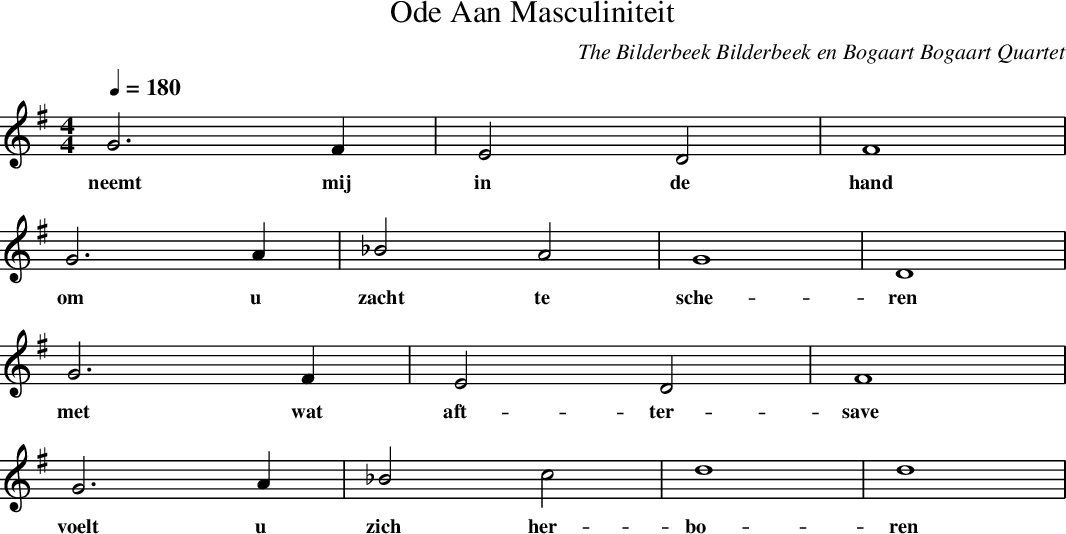
\includegraphics[width=\textwidth,height=\textheight,keepaspectratio]{../songs/03_ode_aan_masculiniteit.png}
  \caption{Ode Aan Masculiniteit}
  \label{fig:03_ode_aan_masculiniteit}
\end{figure}

%%%%%%%%%%%%%%%%%%%%%%%%%%%%%%%%%%%%%%%%%%%%%%%%%%%%%%%%%%%%%%%%%%%%%%%%%%%%%%%%
\section{Het Koffielied}
%%%%%%%%%%%%%%%%%%%%%%%%%%%%%%%%%%%%%%%%%%%%%%%%%%%%%%%%%%%%%%%%%%%%%%%%%%%%%%%%

\lstinputlisting[
  caption = Het Koffielied,
  label = lst:04_het_koffielied
]{../songs/04_het_koffielied.txt}

\begin{figure}[!htbp]
  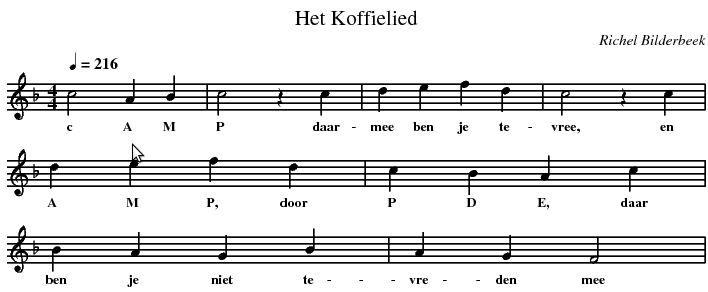
\includegraphics[width=\textwidth,height=\textheight,keepaspectratio]{../songs/04_het_koffielied.png}
  \caption{Het Koffielied}
  \label{fig:04_het_koffielied}
\end{figure}

%%%%%%%%%%%%%%%%%%%%%%%%%%%%%%%%%%%%%%%%%%%%%%%%%%%%%%%%%%%%%%%%%%%%%%%%%%%%%%%%
\section{Hendrik}
%%%%%%%%%%%%%%%%%%%%%%%%%%%%%%%%%%%%%%%%%%%%%%%%%%%%%%%%%%%%%%%%%%%%%%%%%%%%%%%%

\lstinputlisting[
  caption = Hendrik,
  label = lst:05_hendrik
]{../songs/05_hendrik.txt}

\begin{figure}[!htbp]
  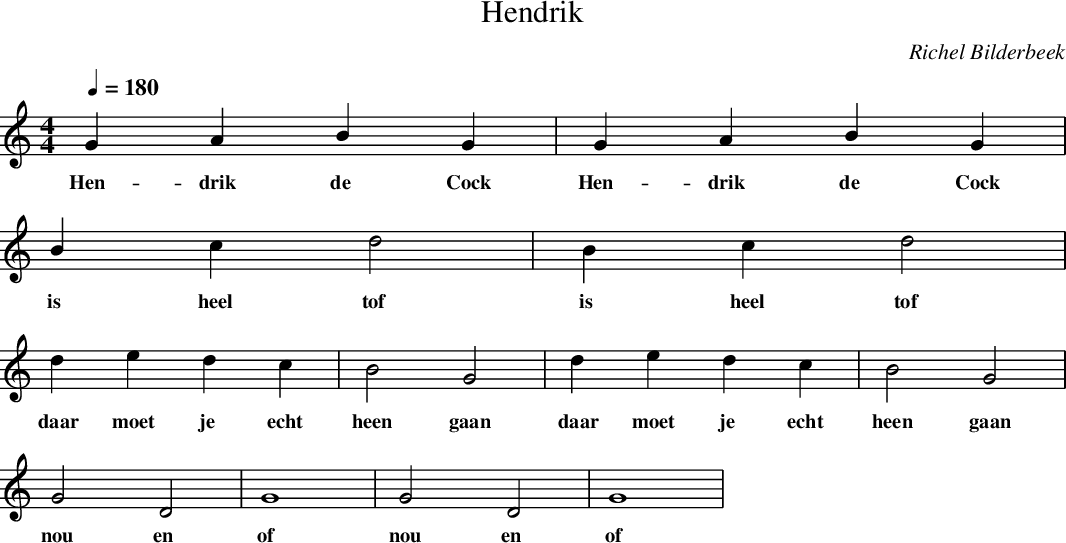
\includegraphics[width=\textwidth,height=\textheight,keepaspectratio]{../songs/05_hendrik.png}
  \caption{Hendrik}
  \label{fig:05_hendrik}
\end{figure}

%%%%%%%%%%%%%%%%%%%%%%%%%%%%%%%%%%%%%%%%%%%%%%%%%%%%%%%%%%%%%%%%%%%%%%%%%%%%%%%%
\section{Leontien}
%%%%%%%%%%%%%%%%%%%%%%%%%%%%%%%%%%%%%%%%%%%%%%%%%%%%%%%%%%%%%%%%%%%%%%%%%%%%%%%%

\lstinputlisting[
  caption = Leontien,
  label = lst:06_leontien
]{../songs/06_leontien.txt}

\begin{figure}[!htbp]
  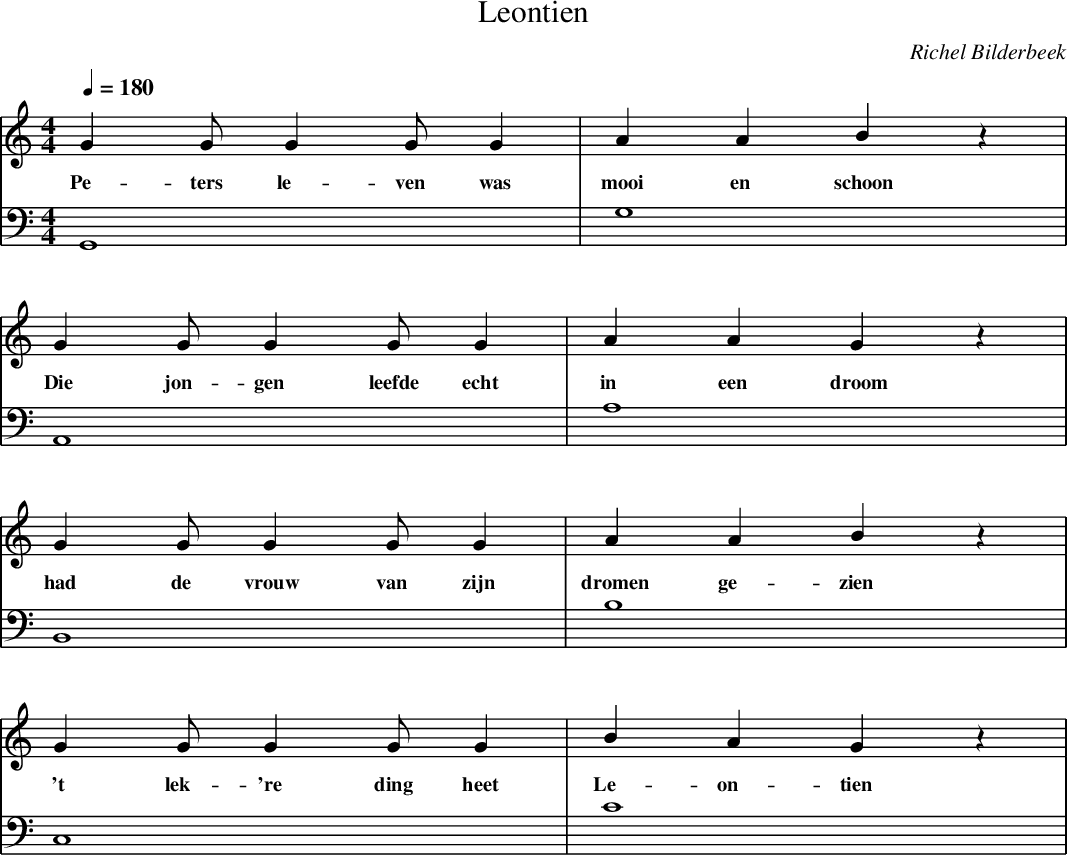
\includegraphics[width=\textwidth,height=\textheight,keepaspectratio]{../songs/06_leontien.png}
  \caption{Leontien}
  \label{fig:06_leontien}
\end{figure}

%%%%%%%%%%%%%%%%%%%%%%%%%%%%%%%%%%%%%%%%%%%%%%%%%%%%%%%%%%%%%%%%%%%%%%%%%%%%%%%%
\chapter{Kinderliefde}
%%%%%%%%%%%%%%%%%%%%%%%%%%%%%%%%%%%%%%%%%%%%%%%%%%%%%%%%%%%%%%%%%%%%%%%%%%%%%%%%

\lstinputlisting[
  caption = Kinderliefde,
  label = lst:07_kinderliefde
]{../songs/07_kinderliefde.txt}

\begin{figure}[!htbp]
  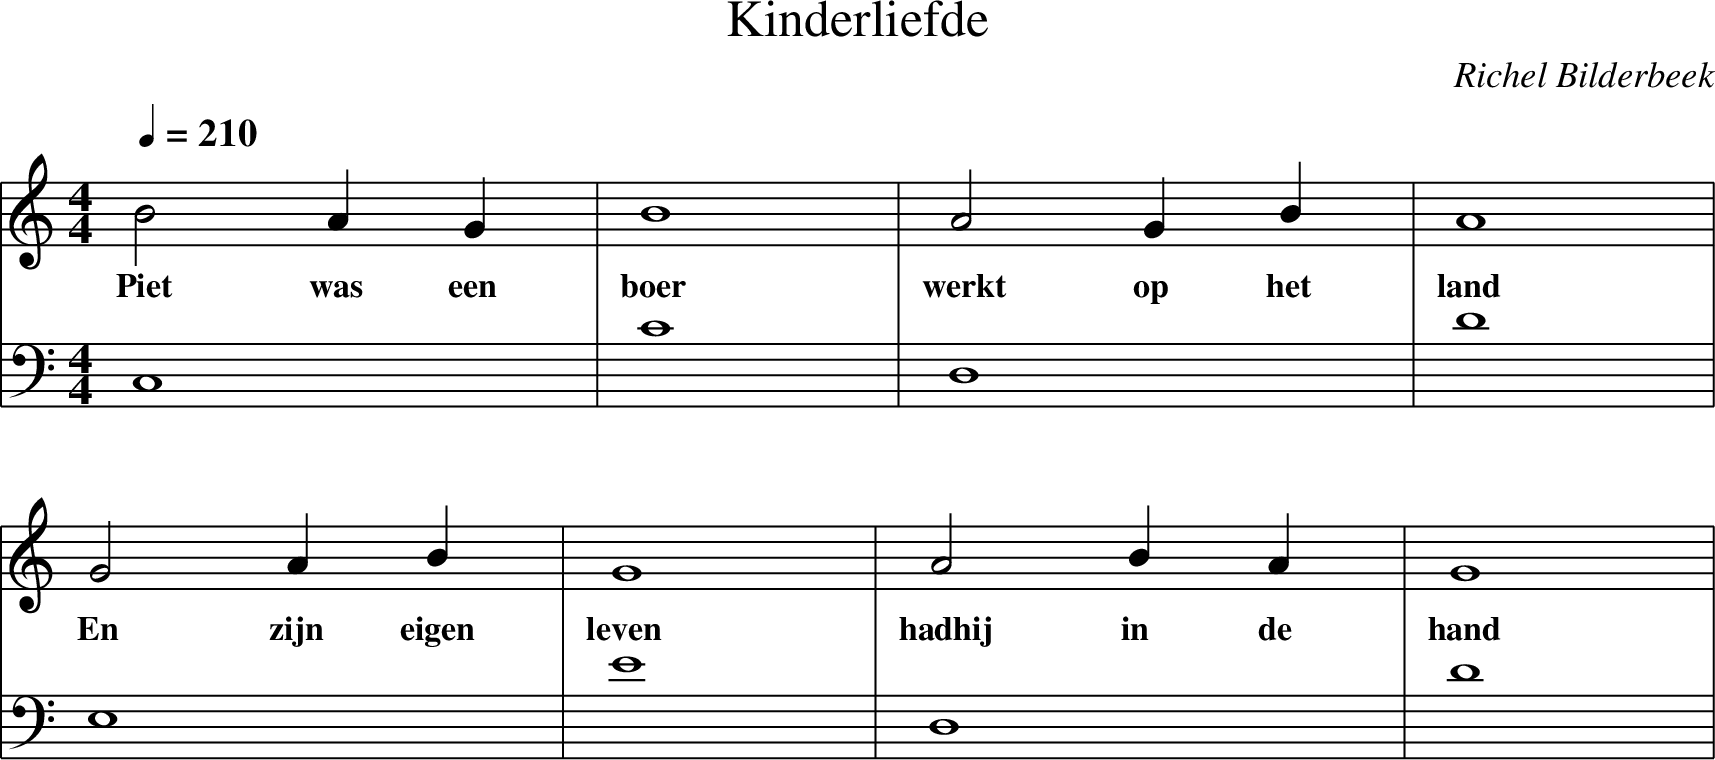
\includegraphics[width=\textwidth,height=\textheight,keepaspectratio]{../songs/07_kinderliefde.png}
  \caption{Kinderliefde}
  \label{fig:07_kinderliefde}
\end{figure}

%%%%%%%%%%%%%%%%%%%%%%%%%%%%%%%%%%%%%%%%%%%%%%%%%%%%%%%%%%%%%%%%%%%%%%%%%%%%%%%%
\chapter{Vroeger}
%%%%%%%%%%%%%%%%%%%%%%%%%%%%%%%%%%%%%%%%%%%%%%%%%%%%%%%%%%%%%%%%%%%%%%%%%%%%%%%%

\lstinputlisting[
  caption = Vroeger,
  label = lst:08_vroeger
]{../songs/08_vroeger.txt}

\begin{figure}[!htbp]
  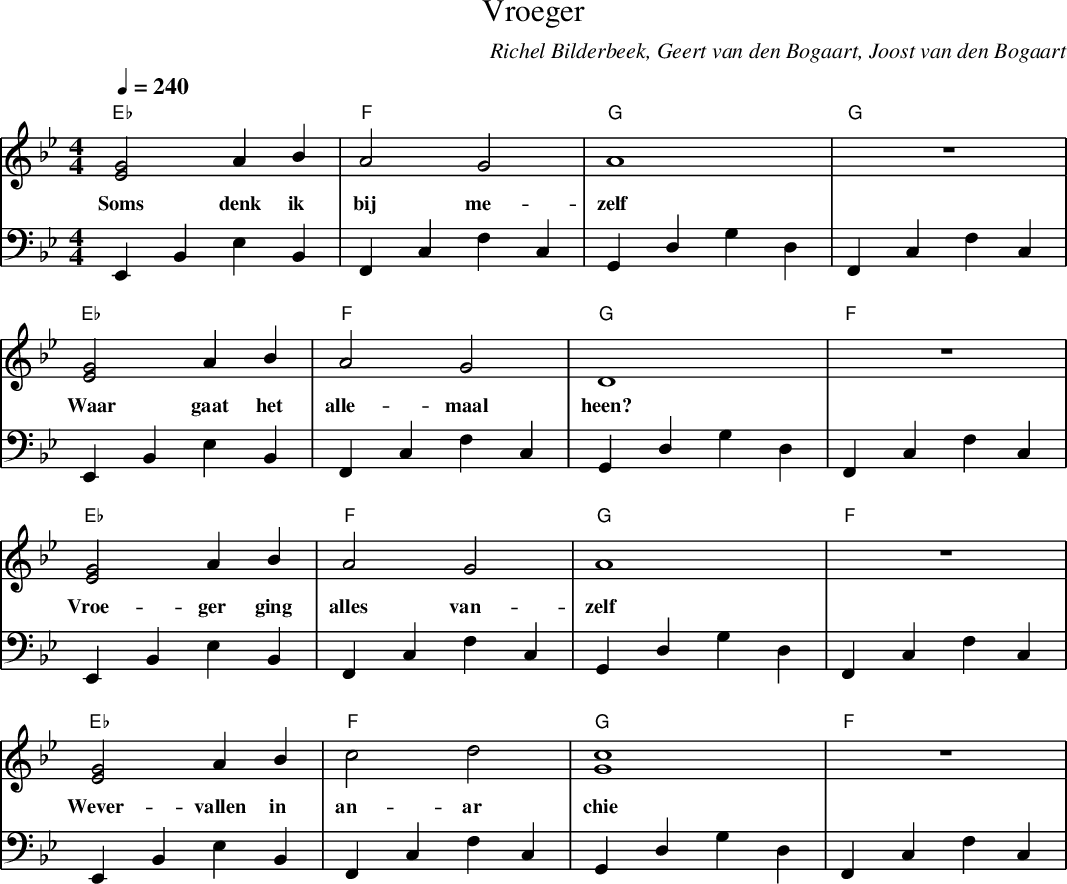
\includegraphics[width=\textwidth,height=\textheight,keepaspectratio]{../songs/08_vroeger.png}
  \caption{Vroeger}
  \label{fig:08_vroeger}
\end{figure}

%%%%%%%%%%%%%%%%%%%%%%%%%%%%%%%%%%%%%%%%%%%%%%%%%%%%%%%%%%%%%%%%%%%%%%%%%%%%%%%%
\chapter{Hendriklied 1}
%%%%%%%%%%%%%%%%%%%%%%%%%%%%%%%%%%%%%%%%%%%%%%%%%%%%%%%%%%%%%%%%%%%%%%%%%%%%%%%%

\lstinputlisting[
  caption = Hendriklied 1,
  label = lst:09_hendriklied_1
]{../songs/09_hendriklied_1.txt}

\begin{figure}[!htbp]
  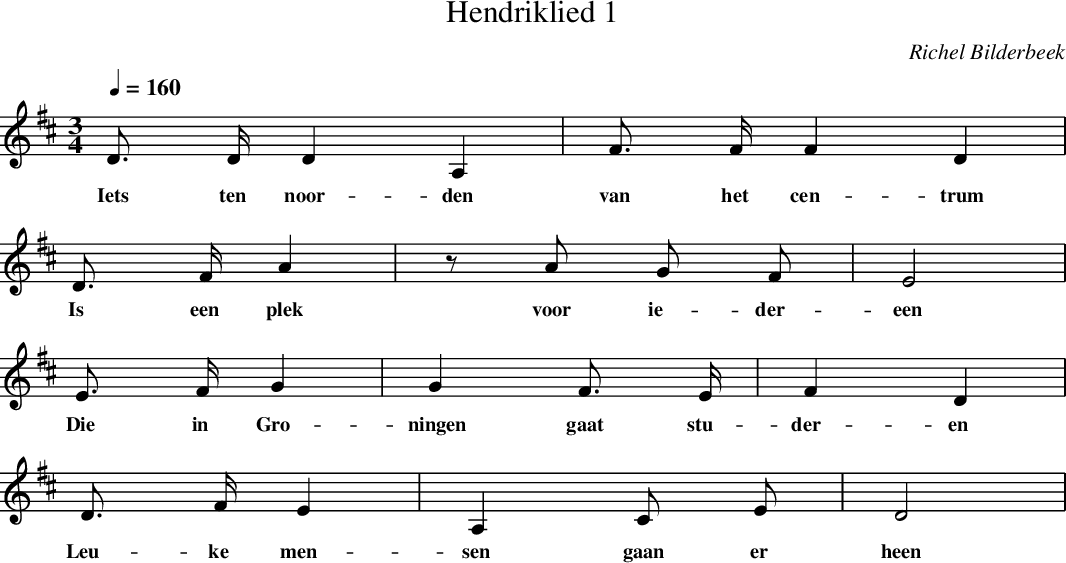
\includegraphics[width=\textwidth,height=\textheight,keepaspectratio]{../songs/09_hendriklied_1.png}
  \caption{Hendriklied 1}
  \label{fig:09_hendriklied_1}
\end{figure}

%%%%%%%%%%%%%%%%%%%%%%%%%%%%%%%%%%%%%%%%%%%%%%%%%%%%%%%%%%%%%%%%%%%%%%%%%%%%%%%%
\section{Hendriklied 2}
%%%%%%%%%%%%%%%%%%%%%%%%%%%%%%%%%%%%%%%%%%%%%%%%%%%%%%%%%%%%%%%%%%%%%%%%%%%%%%%%

\lstinputlisting[
  caption = Hendriklied 2,
  label = lst:10_hendriklied_2
]{../songs/10_hendriklied_2.txt}

%\begin{figure}[!htbp]
%  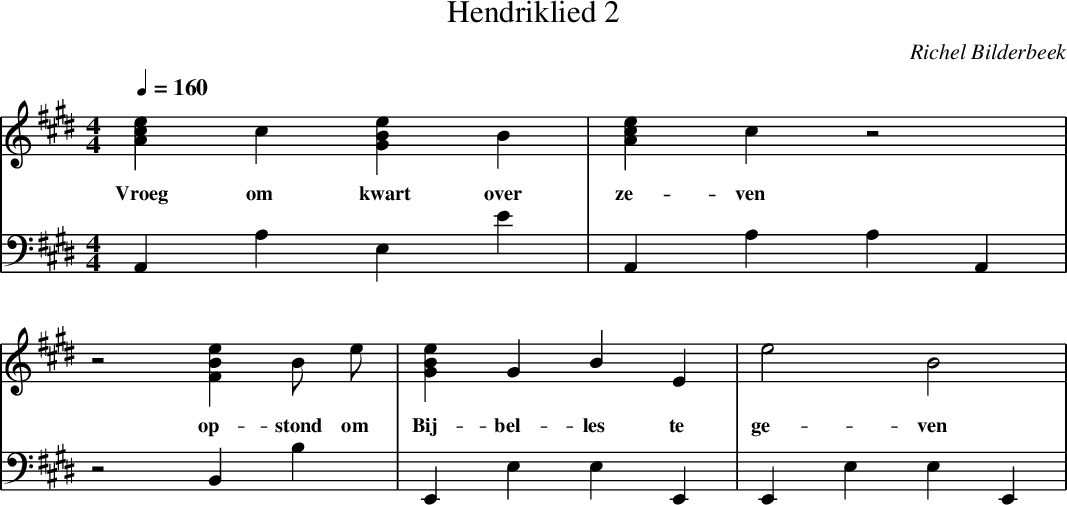
\includegraphics[width=\textwidth,height=\textheight,keepaspectratio]{../songs/10_hendriklied_2.png}
%  \caption{Hendriklied 2}
%  \label{fig:10_hendriklied_2}
%\end{figure}

%%%%%%%%%%%%%%%%%%%%%%%%%%%%%%%%%%%%%%%%%%%%%%%%%%%%%%%%%%%%%%%%%%%%%%%%%%%%%%%%
\section{Rood Geluk}
%%%%%%%%%%%%%%%%%%%%%%%%%%%%%%%%%%%%%%%%%%%%%%%%%%%%%%%%%%%%%%%%%%%%%%%%%%%%%%%%

\lstinputlisting[
  caption = Rood Geluk,
  label = lst:11_rood_geluk
]{../songs/11_rood_geluk.txt}

\begin{figure}[!htbp]
  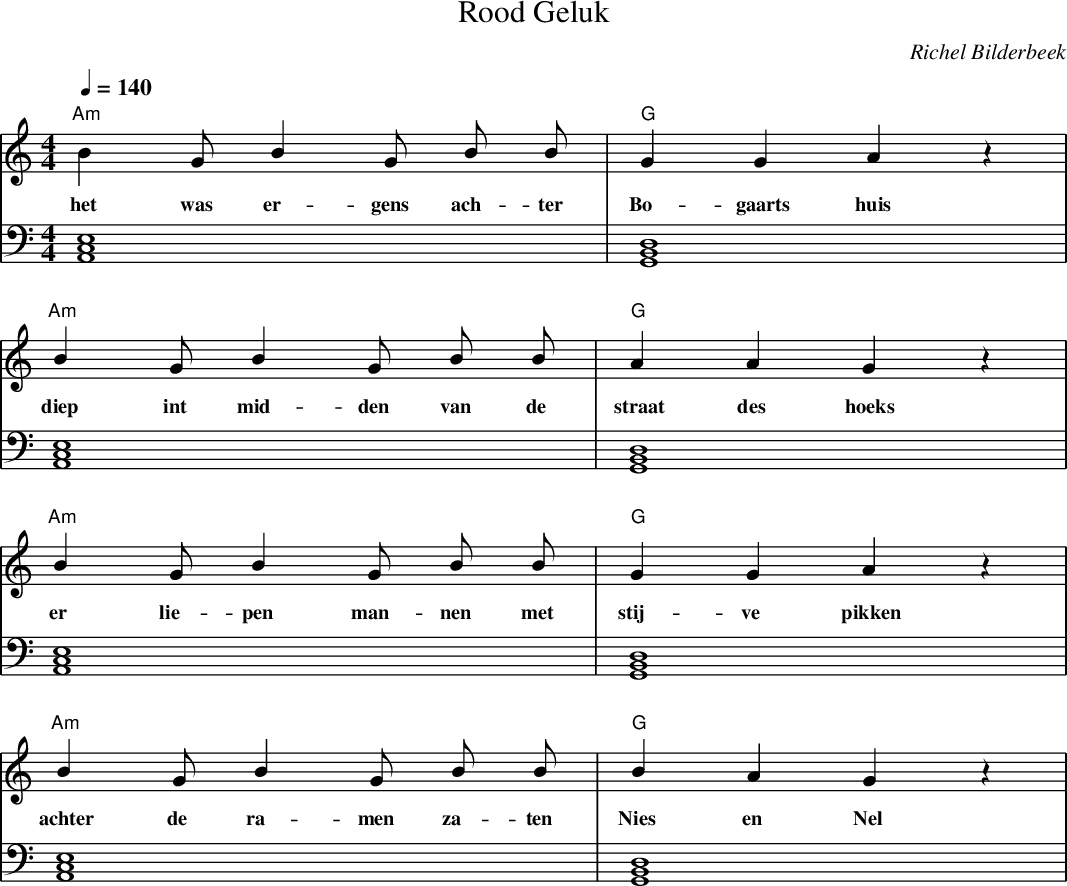
\includegraphics[width=\textwidth,height=\textheight,keepaspectratio]{../songs/11_rood_geluk.png}
  \caption{Rood Geluk}
  \label{fig:11_rood_geluk}
\end{figure}

%%%%%%%%%%%%%%%%%%%%%%%%%%%%%%%%%%%%%%%%%%%%%%%%%%%%%%%%%%%%%%%%%%%%%%%%%%%%%%%%
\section{O, Mooie Geluidsvrouw}
%%%%%%%%%%%%%%%%%%%%%%%%%%%%%%%%%%%%%%%%%%%%%%%%%%%%%%%%%%%%%%%%%%%%%%%%%%%%%%%%

\lstinputlisting[
  caption = O, Mooie Geluidsvrouw,
  label = lst:12_o_mooie_geluidsvrouw
]{../songs/12_o_mooie_geluidsvrouw.txt}

\begin{figure}[!htbp]
  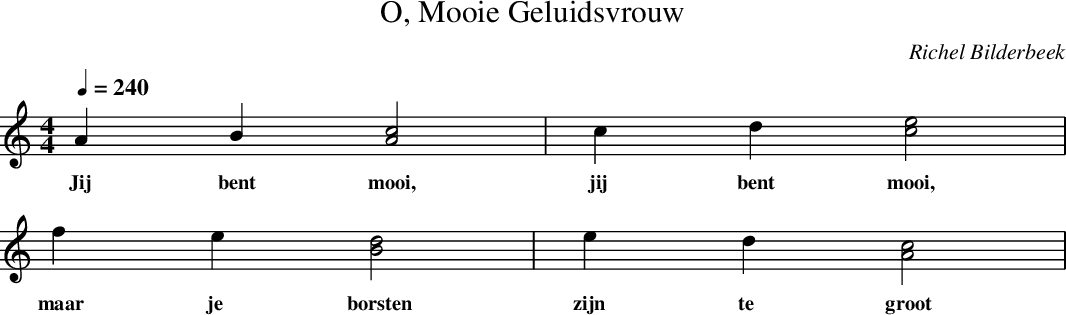
\includegraphics[width=\textwidth,height=\textheight,keepaspectratio]{../songs/12_o_mooie_geluidsvrouw.png}
  \caption{O, Mooie Geluidsvrouw}
  \label{fig:12_o_mooie_geluidsvrouw}
\end{figure}

%%%%%%%%%%%%%%%%%%%%%%%%%%%%%%%%%%%%%%%%%%%%%%%%%%%%%%%%%%%%%%%%%%%%%%%%%%%%%%%%
\section{Hendriklied 3}
%%%%%%%%%%%%%%%%%%%%%%%%%%%%%%%%%%%%%%%%%%%%%%%%%%%%%%%%%%%%%%%%%%%%%%%%%%%%%%%%

\lstinputlisting[
  caption = Hendriklied 3,
  label = lst:13_hendriklied_3
]{../songs/13_hendriklied_3.txt}

\begin{figure}[!htbp]
  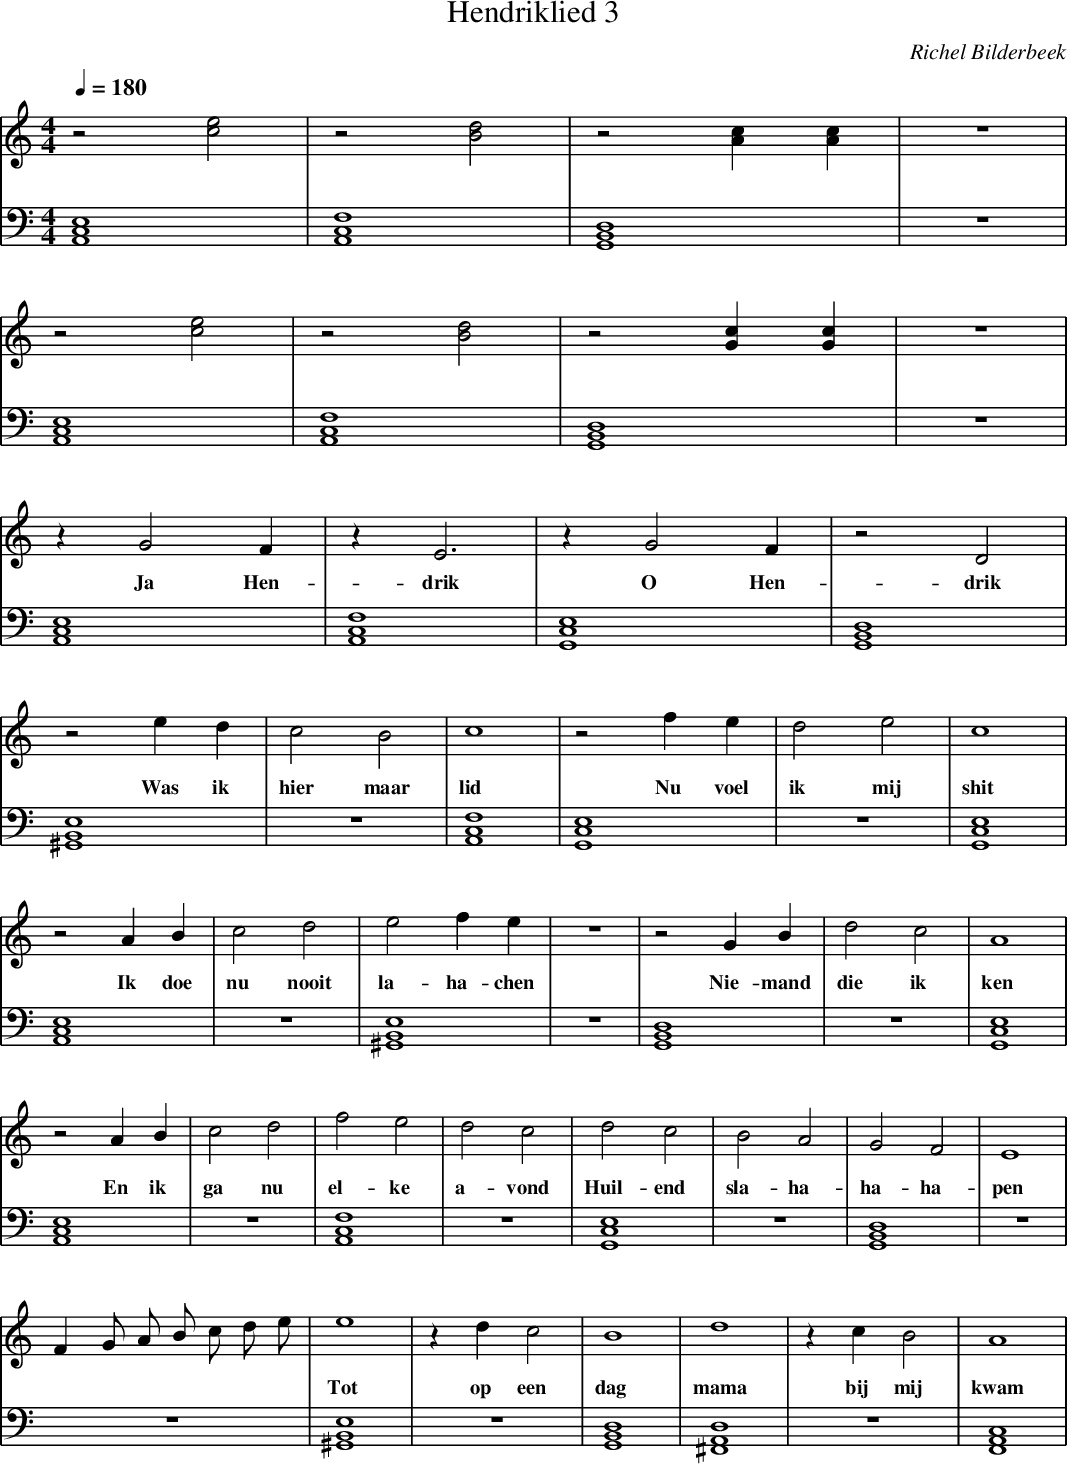
\includegraphics[width=\textwidth,height=\textheight,keepaspectratio]{../songs/13_hendriklied_3-0.png}
  \caption{Hendriklied 3 1/2}
  \label{fig:13_hendriklied_3_1}
\end{figure}

\begin{figure}[!htbp]
  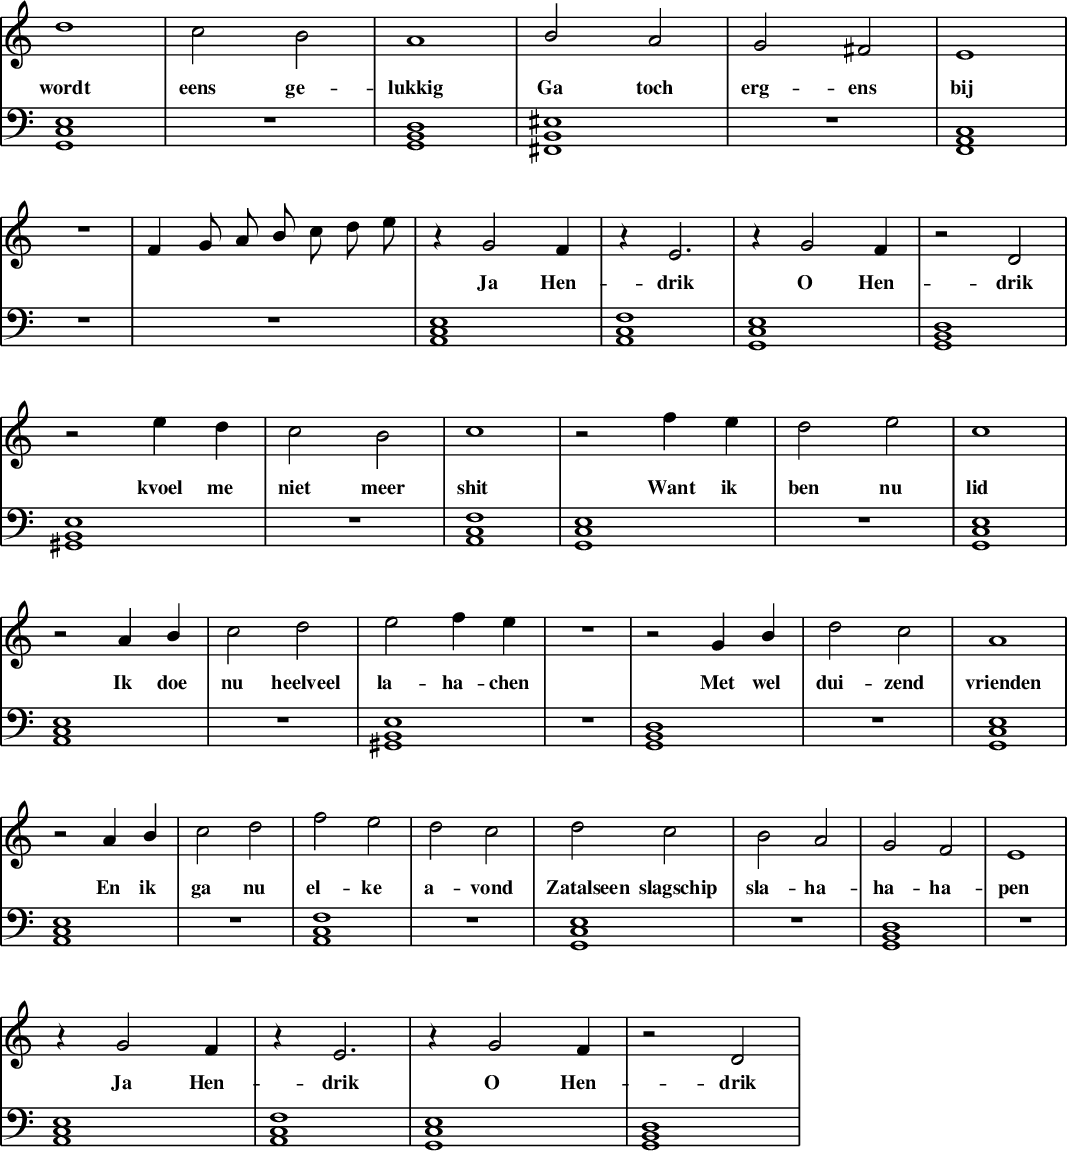
\includegraphics[width=\textwidth,height=\textheight,keepaspectratio]{../songs/13_hendriklied_3-1.png}
  \caption{Hendriklied 3 2/2}
  \label{fig:13_hendriklied_3_2}
\end{figure}

%%%%%%%%%%%%%%%%%%%%%%%%%%%%%%%%%%%%%%%%%%%%%%%%%%%%%%%%%%%%%%%%%%%%%%%%%%%%%%%%
\section{Come Home Darling}
%%%%%%%%%%%%%%%%%%%%%%%%%%%%%%%%%%%%%%%%%%%%%%%%%%%%%%%%%%%%%%%%%%%%%%%%%%%%%%%%

\lstinputlisting[
  caption = Come Home Darling,
  label = lst:14_come_home_darling
]{../songs/14_come_home_darling.txt}

\begin{figure}[!htbp]
  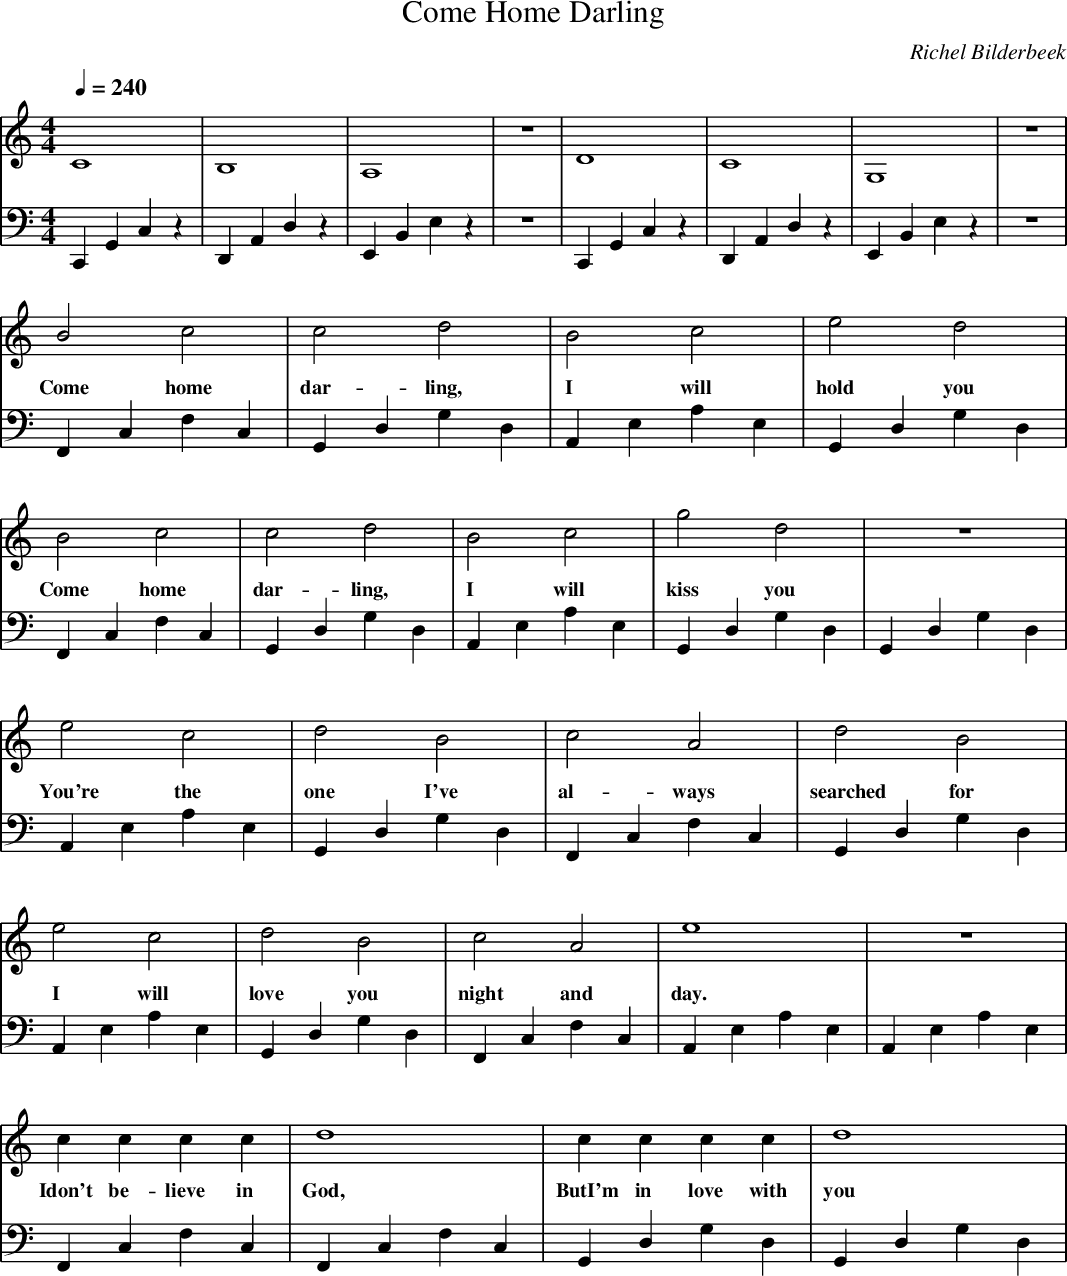
\includegraphics[width=\textwidth,height=\textheight,keepaspectratio]{../songs/14_come_home_darling-0.png}
  \caption{Come Home Darling 1/2}
  \label{fig:14_come_home_darling_1}
\end{figure}

\begin{figure}[!htbp]
  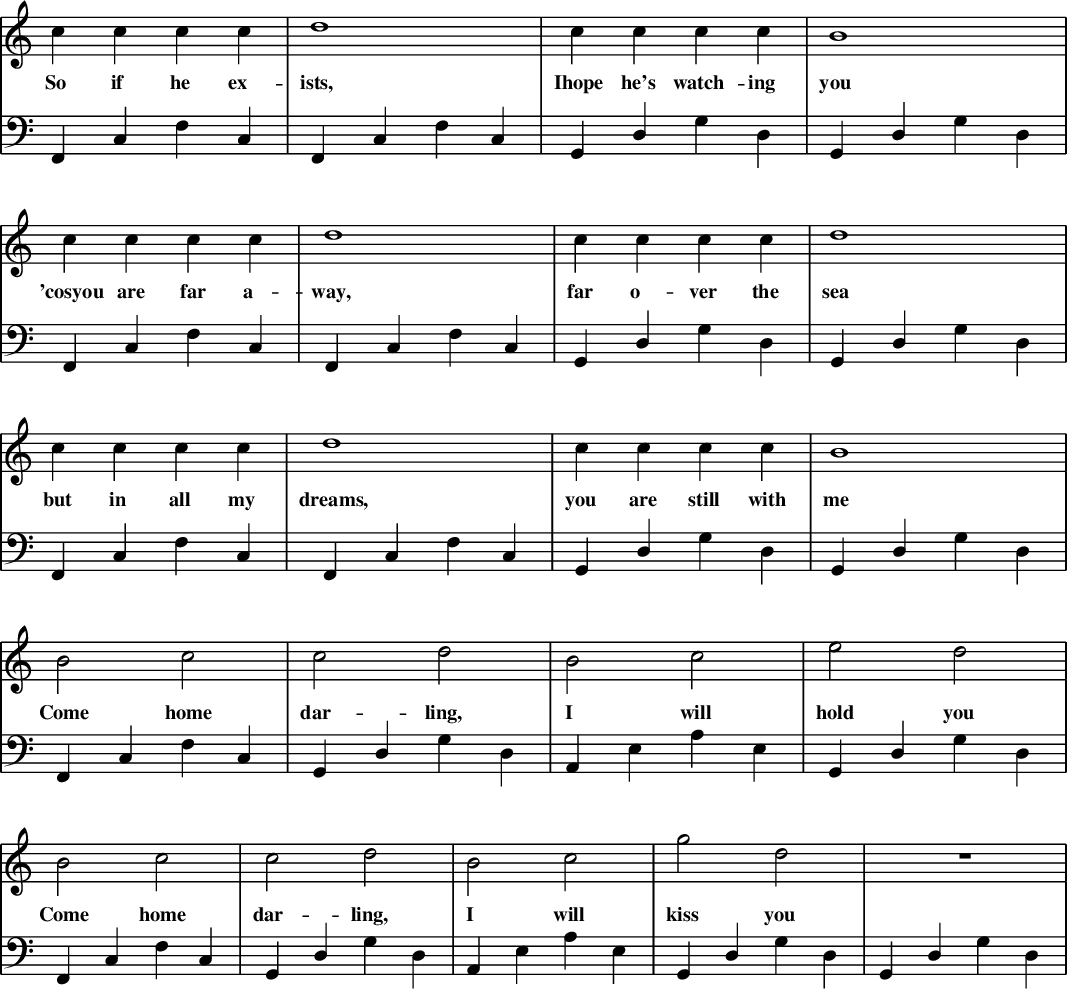
\includegraphics[width=\textwidth,height=\textheight,keepaspectratio]{../songs/14_come_home_darling-1.png}
  \caption{Come Home Darling 2/2}
  \label{fig:14_come_home_darling_2}
\end{figure}

%%%%%%%%%%%%%%%%%%%%%%%%%%%%%%%%%%%%%%%%%%%%%%%%%%%%%%%%%%%%%%%%%%%%%%%%%%%%%%%%
\section{Het Neukmenslied}
%%%%%%%%%%%%%%%%%%%%%%%%%%%%%%%%%%%%%%%%%%%%%%%%%%%%%%%%%%%%%%%%%%%%%%%%%%%%%%%%

\lstinputlisting[
  caption = Het Neukmenslied,
  label = lst:15_het_neukmenslied
]{../songs/15_het_neukmenslied.txt}

\begin{figure}[!htbp]
  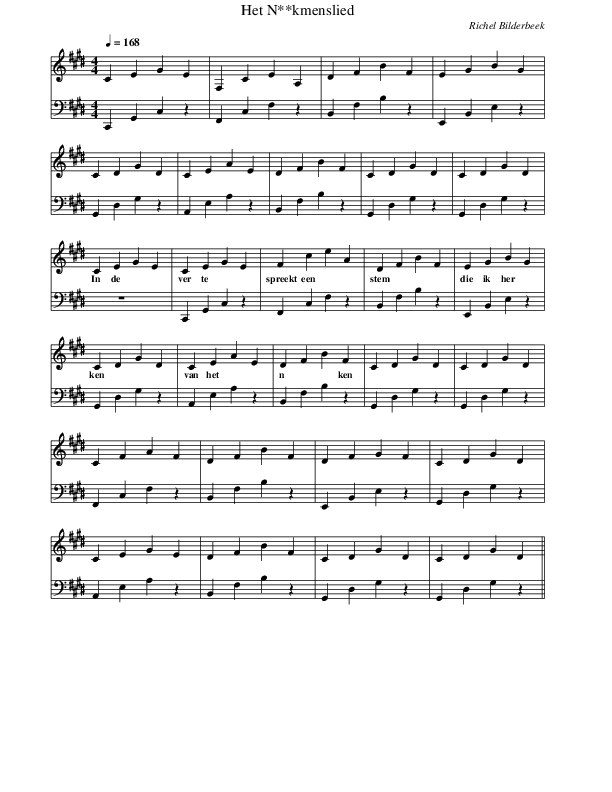
\includegraphics[width=\textwidth,height=\textheight,keepaspectratio]{../songs/15_het_neukmenslied.png}
  \caption{Het Neukmenslied}
  \label{fig:15_het_neukmenslied}
\end{figure}

%%%%%%%%%%%%%%%%%%%%%%%%%%%%%%%%%%%%%%%%%%%%%%%%%%%%%%%%%%%%%%%%%%%%%%%%%%%%%%%%
\section{Het Leven Is Naar}
%%%%%%%%%%%%%%%%%%%%%%%%%%%%%%%%%%%%%%%%%%%%%%%%%%%%%%%%%%%%%%%%%%%%%%%%%%%%%%%%

\lstinputlisting[
  caption = Het Leven Is Naar,
  label = lst:18_het_leven_is_naar
]{../songs/18_het_leven_is_naar.txt}

\begin{figure}[!htbp]
  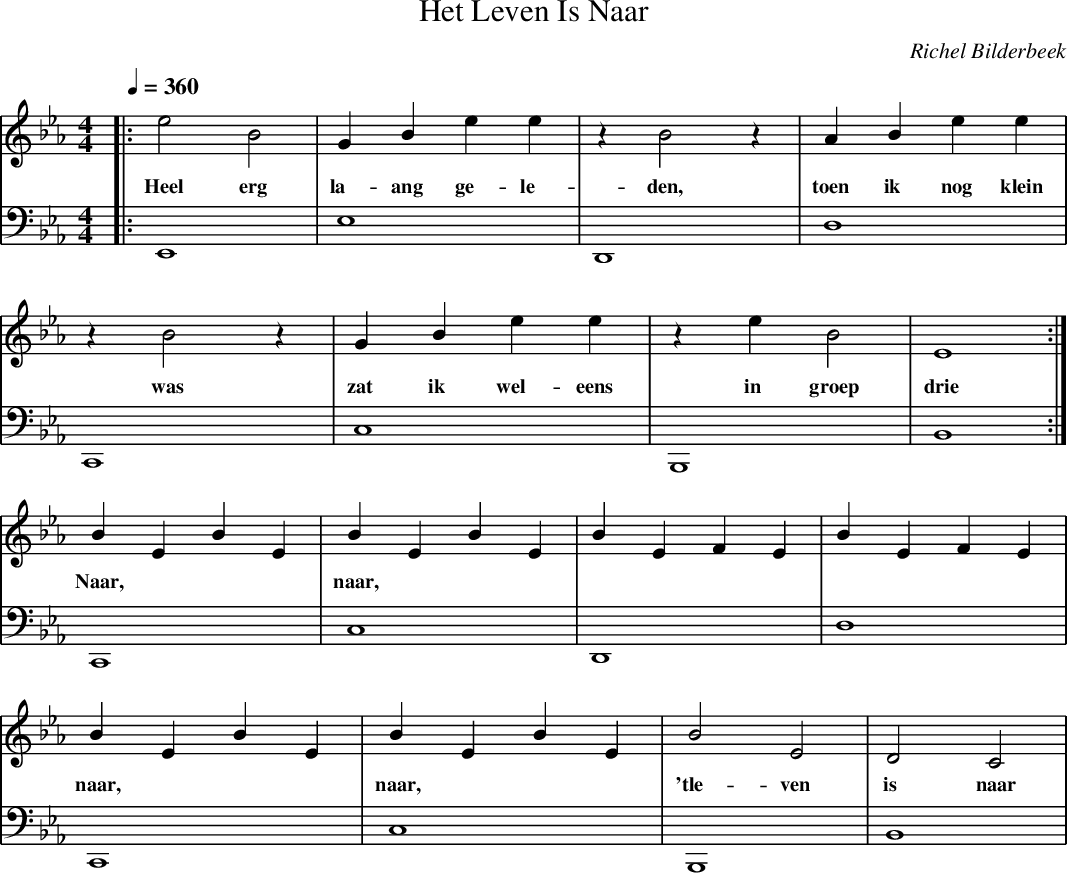
\includegraphics[width=\textwidth,height=\textheight,keepaspectratio]{../songs/18_het_leven_is_naar.png}
  \caption{Het Leven Is Naar}
  \label{fig:18_het_leven_is_naar}
\end{figure}

%%%%%%%%%%%%%%%%%%%%%%%%%%%%%%%%%%%%%%%%%%%%%%%%%%%%%%%%%%%%%%%%%%%%%%%%%%%%%%%%
\section{Hoggamus Higgamus}
%%%%%%%%%%%%%%%%%%%%%%%%%%%%%%%%%%%%%%%%%%%%%%%%%%%%%%%%%%%%%%%%%%%%%%%%%%%%%%%%

\lstinputlisting[
  caption = Hoggamus Higgamus,
  label = lst:17_hoggamus_higgamus
]{../songs/17_hoggamus_higgamus.txt}

% \begin{figure}[!htbp]
%   \includegraphics[width=\textwidth,height=\textheight,keepaspectratio]{../songs/17_hoggamus_higgamus.png}
%   \caption{Hoggamus Higgamus}
%   \label{fig:17_hoggamus_higgamus}
% \end{figure}

%%%%%%%%%%%%%%%%%%%%%%%%%%%%%%%%%%%%%%%%%%%%%%%%%%%%%%%%%%%%%%%%%%%%%%%%%%%%%%%%
\section{Het Leven Is Naar}
%%%%%%%%%%%%%%%%%%%%%%%%%%%%%%%%%%%%%%%%%%%%%%%%%%%%%%%%%%%%%%%%%%%%%%%%%%%%%%%%

\lstinputlisting[
  caption = Het Leven Is Naar,
  label = lst:18_het_leven_is_naar
]{../songs/18_het_leven_is_naar.txt}

\begin{figure}[!htbp]
  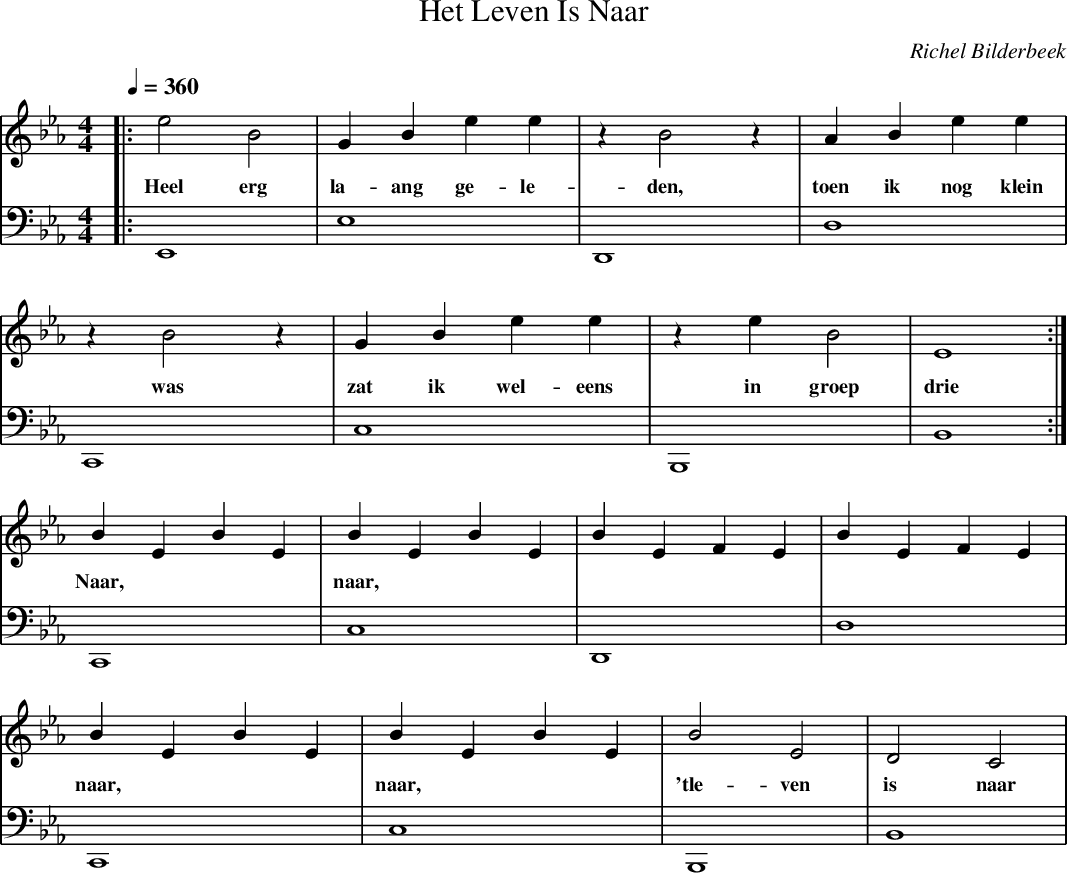
\includegraphics[width=\textwidth,height=\textheight,keepaspectratio]{../songs/18_het_leven_is_naar.png}
  \caption{Het Leven Is Naar}
  \label{fig:18_het_leven_is_naar}
\end{figure}

%%%%%%%%%%%%%%%%%%%%%%%%%%%%%%%%%%%%%%%%%%%%%%%%%%%%%%%%%%%%%%%%%%%%%%%%%%%%%%%%
\section{Het Leven Is Een Vuile Kolerelijer}
%%%%%%%%%%%%%%%%%%%%%%%%%%%%%%%%%%%%%%%%%%%%%%%%%%%%%%%%%%%%%%%%%%%%%%%%%%%%%%%%

\lstinputlisting[
  caption = Het Leven Is Een Vuile Kolerelijer,
  label = lst:19_het_leven_is_een_vuile_kolerelijer
]{../songs/19_het_leven_is_een_vuile_kolerelijer.txt}

%\begin{figure}[!htbp]
%  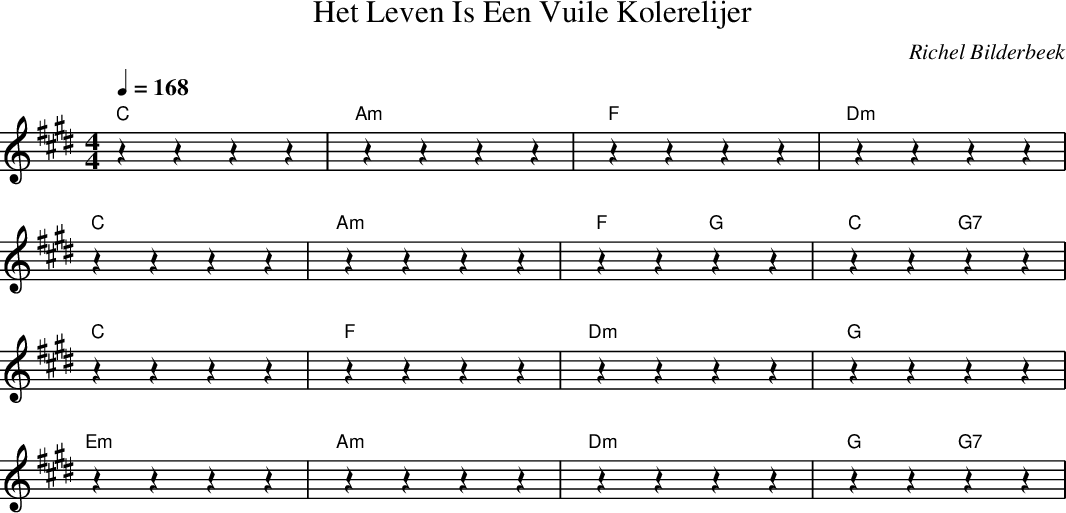
\includegraphics[width=\textwidth,height=\textheight,keepaspectratio]{../songs/19_het_leven_is_een_vuile_kolerelijer.png}
%  \caption{Het Leven Is Een Vuile Kolerelijer}
%  \label{fig:19_het_leven_is_een_vuile_kolerelijer}
%\end{figure}

%%%%%%%%%%%%%%%%%%%%%%%%%%%%%%%%%%%%%%%%%%%%%%%%%%%%%%%%%%%%%%%%%%%%%%%%%%%%%%%%
\section{Al Heb Je Blauw Haar}
%%%%%%%%%%%%%%%%%%%%%%%%%%%%%%%%%%%%%%%%%%%%%%%%%%%%%%%%%%%%%%%%%%%%%%%%%%%%%%%%

\lstinputlisting[
  caption = Al Heb Je Blauw Haar,
  label = lst:20_al_heb_je_blauw_haar
]{../songs/20_al_heb_je_blauw_haar.txt}

\begin{figure}[!htbp]
  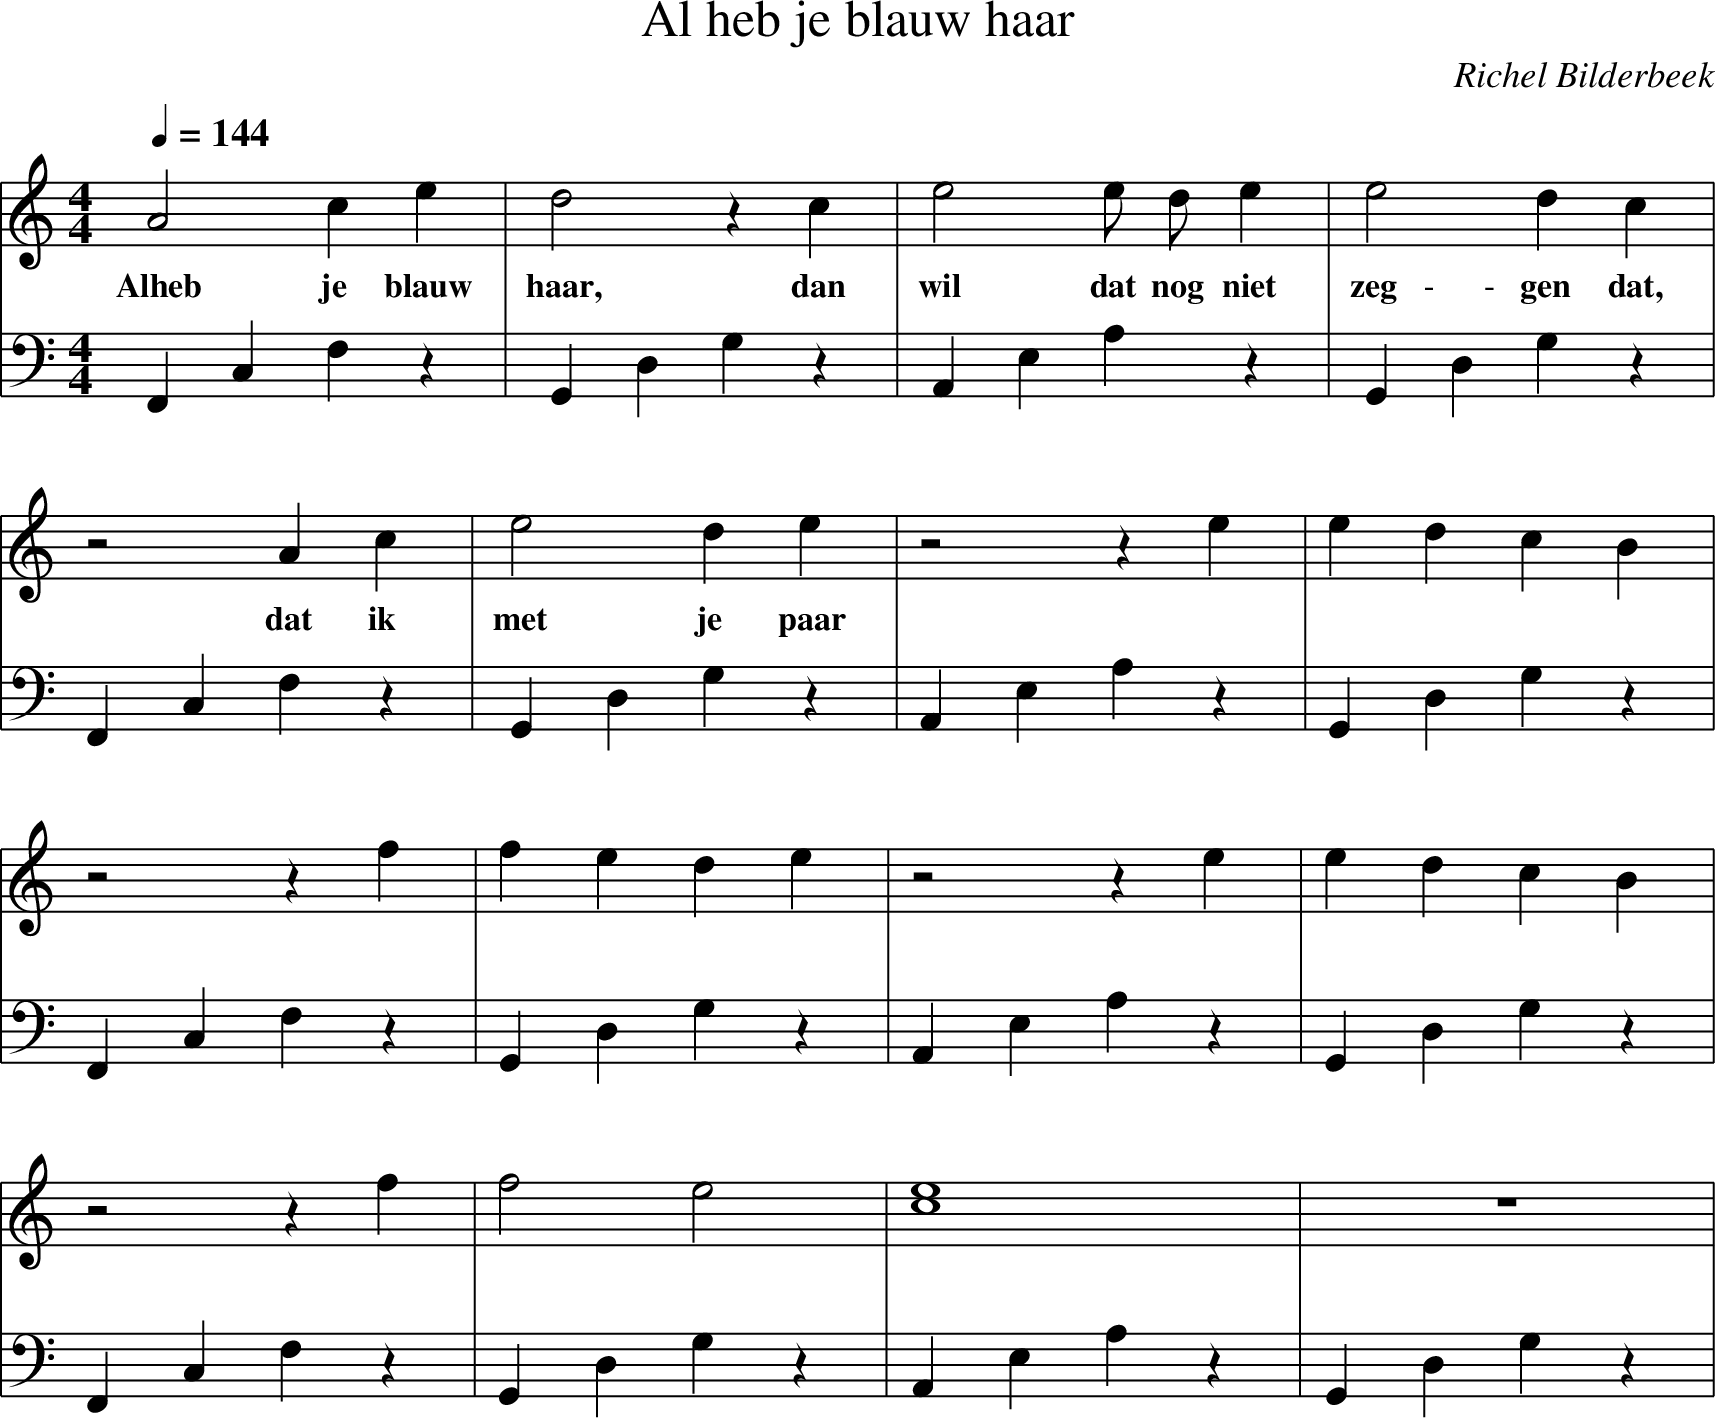
\includegraphics[width=\textwidth,height=\textheight,keepaspectratio]{../songs/20_al_heb_je_blauw_haar.png}
  \caption{Al Heb Je Blauw Haar}
  \label{fig:20_al_heb_je_blauw_haar}
\end{figure}

%%%%%%%%%%%%%%%%%%%%%%%%%%%%%%%%%%%%%%%%%%%%%%%%%%%%%%%%%%%%%%%%%%%%%%%%%%%%%%%%
\chapter{Wooloo Mooloo}
%%%%%%%%%%%%%%%%%%%%%%%%%%%%%%%%%%%%%%%%%%%%%%%%%%%%%%%%%%%%%%%%%%%%%%%%%%%%%%%%

\lstinputlisting[
  caption = Wooloo Mooloo,
  label = lst:21_wooloo_mooloo
]{../songs/21_wooloo_mooloo.txt}

\begin{figure}[!htbp]
  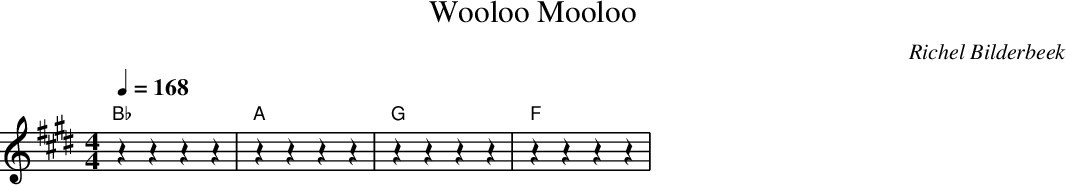
\includegraphics[width=\textwidth,height=\textheight,keepaspectratio]{../songs/21_wooloo_mooloo.png}
  \caption{Wooloo Mooloo}
  \label{fig:21_wooloo_mooloo}
\end{figure}

%%%%%%%%%%%%%%%%%%%%%%%%%%%%%%%%%%%%%%%%%%%%%%%%%%%%%%%%%%%%%%%%%%%%%%%%%%%%%%%%
\section{Mannen}
%%%%%%%%%%%%%%%%%%%%%%%%%%%%%%%%%%%%%%%%%%%%%%%%%%%%%%%%%%%%%%%%%%%%%%%%%%%%%%%%

\lstinputlisting[
  caption = Mannen,
  label = lst:22_mannen
]{../songs/22_mannen.txt}

%\begin{figure}[!htbp]
%  \includegraphics[width=\textwidth,height=\textheight,keepaspectratio]{../songs/22_mannen.png}
%  \caption{Mannen}
%  \label{fig:22_mannen}
%\end{figure}

%%%%%%%%%%%%%%%%%%%%%%%%%%%%%%%%%%%%%%%%%%%%%%%%%%%%%%%%%%%%%%%%%%%%%%%%%%%%%%%%
\section{Slaapliedje}
%%%%%%%%%%%%%%%%%%%%%%%%%%%%%%%%%%%%%%%%%%%%%%%%%%%%%%%%%%%%%%%%%%%%%%%%%%%%%%%%

\lstinputlisting[
  caption = Slaapliedje,
  label = lst:23_slaapliedje
]{../songs/23_slaapliedje.txt}

%\begin{figure}[!htbp]
%  \includegraphics[width=\textwidth,height=\textheight,keepaspectratio]{../songs/23_slaapliedje.png}
%  \caption{Slaapliedje}
%  \label{fig:23_slaapliedje}
%\end{figure}

%%%%%%%%%%%%%%%%%%%%%%%%%%%%%%%%%%%%%%%%%%%%%%%%%%%%%%%%%%%%%%%%%%%%%%%%%%%%%%%%
\section{De Lul}
%%%%%%%%%%%%%%%%%%%%%%%%%%%%%%%%%%%%%%%%%%%%%%%%%%%%%%%%%%%%%%%%%%%%%%%%%%%%%%%%

\lstinputlisting[
  caption = De Lul,
  label = lst:24_de_lul
]{../songs/24_de_lul.txt}

\begin{figure}[!htbp]
  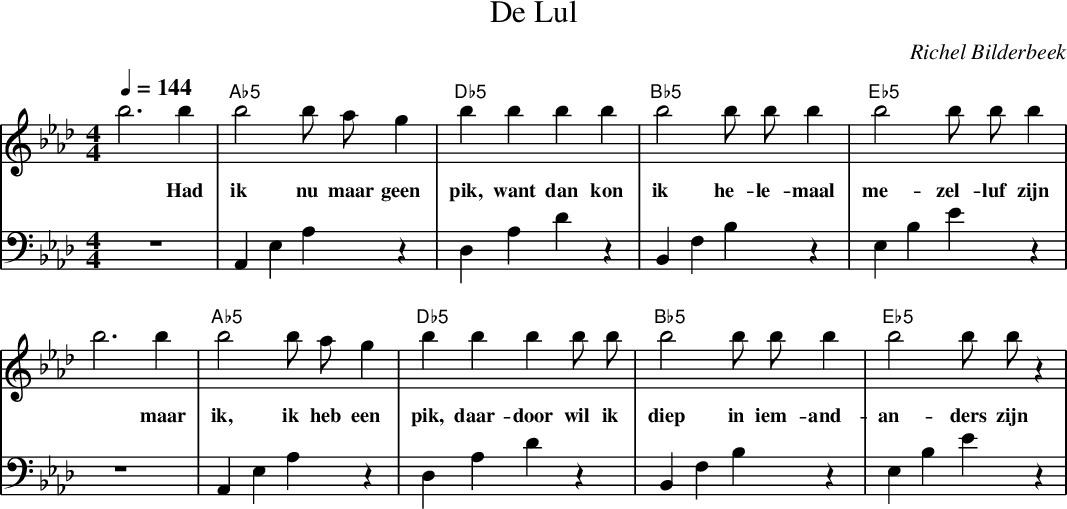
\includegraphics[width=\textwidth,height=\textheight,keepaspectratio]{../songs/24_de_lul.png}
  \caption{De Lul}
  \label{fig:24_de_lul}
\end{figure}

%%%%%%%%%%%%%%%%%%%%%%%%%%%%%%%%%%%%%%%%%%%%%%%%%%%%%%%%%%%%%%%%%%%%%%%%%%%%%%%%
\chapter{Blauw}
%%%%%%%%%%%%%%%%%%%%%%%%%%%%%%%%%%%%%%%%%%%%%%%%%%%%%%%%%%%%%%%%%%%%%%%%%%%%%%%%

\lstinputlisting[
  caption = Blauw,
  label = lst:25_blauw
]{../songs/25_blauw.txt}

%\begin{figure}[!htbp]
%  \includegraphics[width=\textwidth,height=\textheight,keepaspectratio]{../songs/25_blauw.png}
%  \caption{Blauw}
%  \label{fig:25_blauw}
%\end{figure}

%%%%%%%%%%%%%%%%%%%%%%%%%%%%%%%%%%%%%%%%%%%%%%%%%%%%%%%%%%%%%%%%%%%%%%%%%%%%%%%%
\chapter{Morgenvroeg}
%%%%%%%%%%%%%%%%%%%%%%%%%%%%%%%%%%%%%%%%%%%%%%%%%%%%%%%%%%%%%%%%%%%%%%%%%%%%%%%%

\lstinputlisting[
  caption = Morgenvroeg,
  label = lst:26_morgenvroeg
]{../songs/26_morgenvroeg.txt}

%\begin{figure}[!htbp]
%  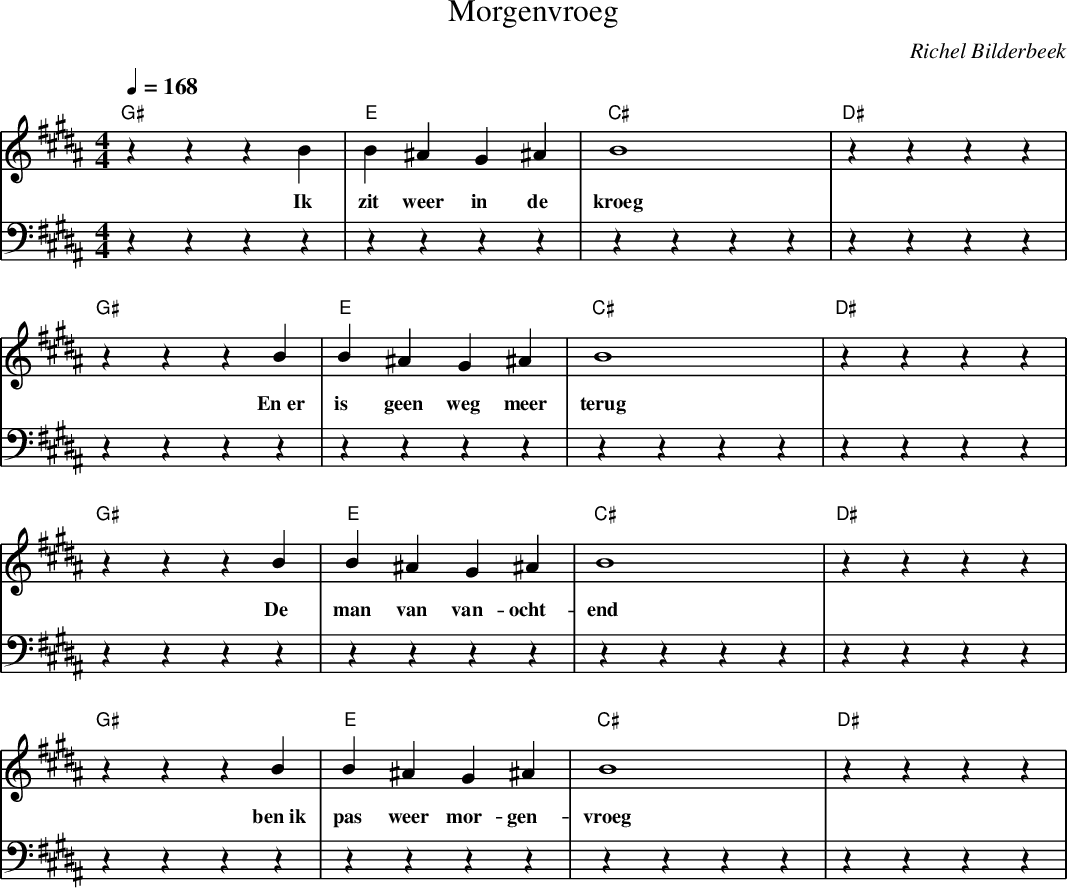
\includegraphics[width=\textwidth,height=\textheight,keepaspectratio]{../songs/26_morgenvroeg.png}
%  \caption{Morgenvroeg}
%  \label{fig:26_morgenvroeg}
%\end{figure}

%%%%%%%%%%%%%%%%%%%%%%%%%%%%%%%%%%%%%%%%%%%%%%%%%%%%%%%%%%%%%%%%%%%%%%%%%%%%%%%%
\section{Zonder Jou Weg}
%%%%%%%%%%%%%%%%%%%%%%%%%%%%%%%%%%%%%%%%%%%%%%%%%%%%%%%%%%%%%%%%%%%%%%%%%%%%%%%%

\lstinputlisting[
  caption = Zonder Jou Weg,
  label = lst:27_zonder_jou_weg
]{../songs/27_zonder_jou_weg.txt}

%\begin{figure}[!htbp]
%  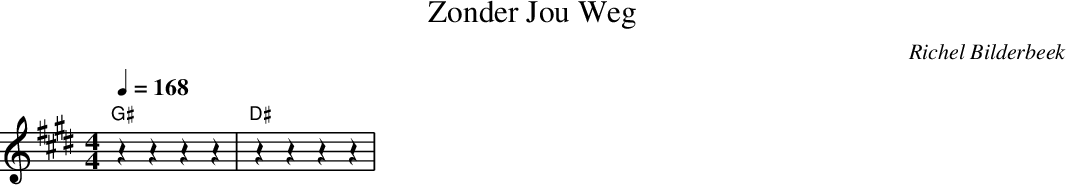
\includegraphics[width=\textwidth,height=\textheight,keepaspectratio]{../songs/27_zonder_jou_weg.png}
%  \caption{Zonder Jou Weg}
%  \label{fig:27_zonder_jou_weg}
%\end{figure}

%%%%%%%%%%%%%%%%%%%%%%%%%%%%%%%%%%%%%%%%%%%%%%%%%%%%%%%%%%%%%%%%%%%%%%%%%%%%%%%%
\section{Klavierstückchen}
%%%%%%%%%%%%%%%%%%%%%%%%%%%%%%%%%%%%%%%%%%%%%%%%%%%%%%%%%%%%%%%%%%%%%%%%%%%%%%%%

\lstinputlisting[
  caption = Klavierstückchen,
  label = lst:28_klavierstueckchen
]{../songs/28_klavierstueckchen.txt}

%\begin{figure}[!htbp]
%  \includegraphics[width=\textwidth,height=\textheight,keepaspectratio]{../songs/28_klavierstueckchen.png}
%  \caption{Klavierstückchen}
%  \label{fig:28_klavierstueckchen}
%\end{figure}

%%%%%%%%%%%%%%%%%%%%%%%%%%%%%%%%%%%%%%%%%%%%%%%%%%%%%%%%%%%%%%%%%%%%%%%%%%%%%%%%
\section{Dortmund}
%%%%%%%%%%%%%%%%%%%%%%%%%%%%%%%%%%%%%%%%%%%%%%%%%%%%%%%%%%%%%%%%%%%%%%%%%%%%%%%%

\lstinputlisting[
  caption = Dortmund,
  label = lst:29_dortmund
]{../songs/29_dortmund.txt}

%\begin{figure}[!htbp]
%  \includegraphics[width=\textwidth,height=\textheight,keepaspectratio]{../songs/29_dortmund.png}
%  \caption{Dortmund}
%  \label{fig:29_dortmund}
%\end{figure}

%%%%%%%%%%%%%%%%%%%%%%%%%%%%%%%%%%%%%%%%%%%%%%%%%%%%%%%%%%%%%%%%%%%%%%%%%%%%%%%%
\section{Die Rolltreppe Und Ich}
%%%%%%%%%%%%%%%%%%%%%%%%%%%%%%%%%%%%%%%%%%%%%%%%%%%%%%%%%%%%%%%%%%%%%%%%%%%%%%%%

\lstinputlisting[
  caption = Die Rolltreppe Und Ich,
  label = lst:30_die_rolltreppe_und_ich
]{../songs/30_die_rolltreppe_und_ich.txt}

%\begin{figure}[!htbp]
%  \includegraphics[width=\textwidth,height=\textheight,keepaspectratio]{../songs/30_die_rolltreppe_und_ich.png}
%  \caption{Die Rolltreppe Und Ich}
%  \label{fig:30_die_rolltreppe_und_ich}
%\end{figure}

%%%%%%%%%%%%%%%%%%%%%%%%%%%%%%%%%%%%%%%%%%%%%%%%%%%%%%%%%%%%%%%%%%%%%%%%%%%%%%%%
\chapter{Blau}
%%%%%%%%%%%%%%%%%%%%%%%%%%%%%%%%%%%%%%%%%%%%%%%%%%%%%%%%%%%%%%%%%%%%%%%%%%%%%%%%

\lstinputlisting[
  caption = Blau,
  label = lst:31_blau
]{../songs/31_blau.txt}

%\begin{figure}[!htbp]
%  \includegraphics[width=\textwidth,height=\textheight,keepaspectratio]{../songs/31_blau.png}
%  \caption{Blau}
%  \label{fig:31_blau}
%\end{figure}

%%%%%%%%%%%%%%%%%%%%%%%%%%%%%%%%%%%%%%%%%%%%%%%%%%%%%%%%%%%%%%%%%%%%%%%%%%%%%%%%
\section{Kaesemond}
%%%%%%%%%%%%%%%%%%%%%%%%%%%%%%%%%%%%%%%%%%%%%%%%%%%%%%%%%%%%%%%%%%%%%%%%%%%%%%%%

\lstinputlisting[
  caption = Kaesemond,
  label = lst:32_kaesemond
]{../songs/32_kaesemond.txt}

%\begin{figure}[!htbp]
%  \includegraphics[width=\textwidth,height=\textheight,keepaspectratio]{../songs/32_kaesemond.png}
%  \caption{Kaesemond}
%  \label{fig:32_kaesemond}
%\end{figure}

%%%%%%%%%%%%%%%%%%%%%%%%%%%%%%%%%%%%%%%%%%%%%%%%%%%%%%%%%%%%%%%%%%%%%%%%%%%%%%%%
\chapter{Wooloo Mooloo (DE)}
%%%%%%%%%%%%%%%%%%%%%%%%%%%%%%%%%%%%%%%%%%%%%%%%%%%%%%%%%%%%%%%%%%%%%%%%%%%%%%%%

\lstinputlisting[
  caption = Wooloo Mooloo (DE),
  label = lst:33_wooloo_mooloo_de
]{../songs/33_wooloo_mooloo_de.txt}

%\begin{figure}[!htbp]
%  \includegraphics[width=\textwidth,height=\textheight,keepaspectratio]{../songs/33_wooloo_mooloo_de.png}
%  \caption{Wooloo Mooloo (DE)}
%  \label{fig:33_wooloo_mooloo_de}
%\end{figure}

%%%%%%%%%%%%%%%%%%%%%%%%%%%%%%%%%%%%%%%%%%%%%%%%%%%%%%%%%%%%%%%%%%%%%%%%%%%%%%%%
\chapter{Morgonsfrueh}
%%%%%%%%%%%%%%%%%%%%%%%%%%%%%%%%%%%%%%%%%%%%%%%%%%%%%%%%%%%%%%%%%%%%%%%%%%%%%%%%

\lstinputlisting[
  caption = Morgonsfrueh,
  label = lst:34_morgensfrueh
]{../songs/34_morgensfrueh.txt}

%\begin{figure}[!htbp]
%  \includegraphics[width=\textwidth,height=\textheight,keepaspectratio]{../songs/34_morgensfrueh.png}
%  \caption{Morgonsfrueh}
%  \label{fig:34_morgensfrueh}
%\end{figure}

%%%%%%%%%%%%%%%%%%%%%%%%%%%%%%%%%%%%%%%%%%%%%%%%%%%%%%%%%%%%%%%%%%%%%%%%%%%%%%%%
\chapter{Wenn Du Haettest Blaue Haare}
%%%%%%%%%%%%%%%%%%%%%%%%%%%%%%%%%%%%%%%%%%%%%%%%%%%%%%%%%%%%%%%%%%%%%%%%%%%%%%%%

\lstinputlisting[
  caption = Wenn Du Haettest Blaue Haare,
  label = lst:35_wenn_du_haettest_blaue_haare
]{../songs/35_wenn_du_haettest_blaue_haare.txt}

%\begin{figure}[!htbp]
%  \includegraphics[width=\textwidth,height=\textheight,keepaspectratio]{../songs/35_wenn_du_haettest_blaue_haare.png}
%  \caption{Wenn Du Haettest Blaue Haare}
%  \label{fig:35_wenn_du_haettest_blaue_haare}
%\end{figure}

%%%%%%%%%%%%%%%%%%%%%%%%%%%%%%%%%%%%%%%%%%%%%%%%%%%%%%%%%%%%%%%%%%%%%%%%%%%%%%%%
\chapter{Der Schwanz}
%%%%%%%%%%%%%%%%%%%%%%%%%%%%%%%%%%%%%%%%%%%%%%%%%%%%%%%%%%%%%%%%%%%%%%%%%%%%%%%%

\lstinputlisting[
  caption = Der Schwanz,
  label = lst:36_der_schwanz
]{../songs/36_der_schwanz.txt}

%\begin{figure}[!htbp]
%  \includegraphics[width=\textwidth,height=\textheight,keepaspectratio]{../songs/36_der_schwanz.png}
%  \caption{Der Schwanz}
%  \label{fig:36_der_schwanz}
%\end{figure}

%%%%%%%%%%%%%%%%%%%%%%%%%%%%%%%%%%%%%%%%%%%%%%%%%%%%%%%%%%%%%%%%%%%%%%%%%%%%%%%%
\chapter{Das Fickmenschlied}
%%%%%%%%%%%%%%%%%%%%%%%%%%%%%%%%%%%%%%%%%%%%%%%%%%%%%%%%%%%%%%%%%%%%%%%%%%%%%%%%

\lstinputlisting[
  caption = Das Fickmenschlied,
  label = lst:37_das_fickmenschlied
]{../songs/37_das_fickmenschlied.txt}

%\begin{figure}[!htbp]
%  \includegraphics[width=\textwidth,height=\textheight,keepaspectratio]{../songs/37_das_fickmenschlied.png}
%  \caption{Das Fickmenschlied}
%  \label{fig:37_das_fickmenschlied}
%\end{figure}

%%%%%%%%%%%%%%%%%%%%%%%%%%%%%%%%%%%%%%%%%%%%%%%%%%%%%%%%%%%%%%%%%%%%%%%%%%%%%%%%
\chapter{Das Leben Ist Mist}
%%%%%%%%%%%%%%%%%%%%%%%%%%%%%%%%%%%%%%%%%%%%%%%%%%%%%%%%%%%%%%%%%%%%%%%%%%%%%%%%

\lstinputlisting[
  caption = Das Leben Ist Mist,
  label = lst:38_das_leben_ist_mist
]{../songs/38_das_leben_ist_mist.txt}

%\begin{figure}[!htbp]
%  \includegraphics[width=\textwidth,height=\textheight,keepaspectratio]{../songs/38_das_leben_ist_mist.png}
%  \caption{Das Leben Ist Mist}
%  \label{fig:38_das_leben_ist_mist}
%\end{figure}

%%%%%%%%%%%%%%%%%%%%%%%%%%%%%%%%%%%%%%%%%%%%%%%%%%%%%%%%%%%%%%%%%%%%%%%%%%%%%%%%
\section{Das Kaffeelied}
%%%%%%%%%%%%%%%%%%%%%%%%%%%%%%%%%%%%%%%%%%%%%%%%%%%%%%%%%%%%%%%%%%%%%%%%%%%%%%%%

\lstinputlisting[
  caption = Das Kaffeelied,
  label = lst:39_das_kaffeelied
]{../songs/39_das_kaffeelied.txt}

%\begin{figure}[!htbp]
%  \includegraphics[width=\textwidth,height=\textheight,keepaspectratio]{../songs/39_das_kaffeelied.png}
%  \caption{Das Kaffeelied}
%  \label{fig:39_das_kaffeelied}
%\end{figure}

%%%%%%%%%%%%%%%%%%%%%%%%%%%%%%%%%%%%%%%%%%%%%%%%%%%%%%%%%%%%%%%%%%%%%%%%%%%%%%%%
\section{The Clifton Suspension Bridge}
%%%%%%%%%%%%%%%%%%%%%%%%%%%%%%%%%%%%%%%%%%%%%%%%%%%%%%%%%%%%%%%%%%%%%%%%%%%%%%%%

\lstinputlisting[
  caption = The Clifton Suspension Bridge,
  label = lst:40_the_clifton_suspension_bridge
]{../songs/40_the_clifton_suspension_bridge.txt}

%\begin{figure}[!htbp]
%  \includegraphics[width=\textwidth,height=\textheight,keepaspectratio]{../songs/40_the_clifton_suspension_bridge.png}
%  \caption{The Clifton Suspension Bridge}
%  \label{fig:40_the_clifton_suspension_bridge}
%\end{figure}

%%%%%%%%%%%%%%%%%%%%%%%%%%%%%%%%%%%%%%%%%%%%%%%%%%%%%%%%%%%%%%%%%%%%%%%%%%%%%%%%
\chapter{You And Me}
%%%%%%%%%%%%%%%%%%%%%%%%%%%%%%%%%%%%%%%%%%%%%%%%%%%%%%%%%%%%%%%%%%%%%%%%%%%%%%%%

\lstinputlisting[
  caption = You And Me,
  label = lst:41_you_and_me
]{../songs/41_you_and_me.txt}

\begin{figure}[!htbp]
  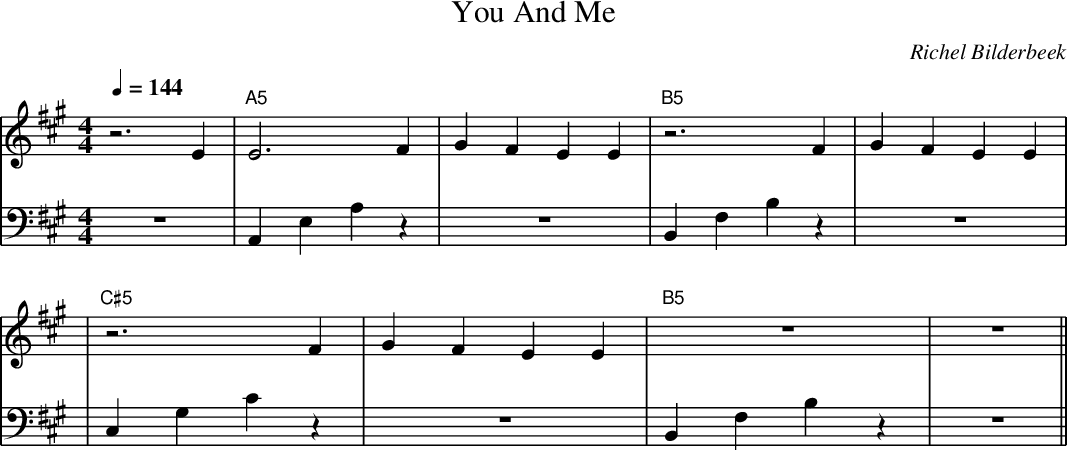
\includegraphics[width=\textwidth,height=\textheight,keepaspectratio]{../songs/41_you_and_me.png}
  \caption{You And Me}
  \label{fig:41_you_and_me}
\end{figure}

%%%%%%%%%%%%%%%%%%%%%%%%%%%%%%%%%%%%%%%%%%%%%%%%%%%%%%%%%%%%%%%%%%%%%%%%%%%%%%%%
\section{To The Pub}
%%%%%%%%%%%%%%%%%%%%%%%%%%%%%%%%%%%%%%%%%%%%%%%%%%%%%%%%%%%%%%%%%%%%%%%%%%%%%%%%

\lstinputlisting[
  caption = To The Pub,
  label = lst:42_to_the_pub
]{../songs/42_to_the_pub.txt}

%\begin{figure}[!htbp]
%  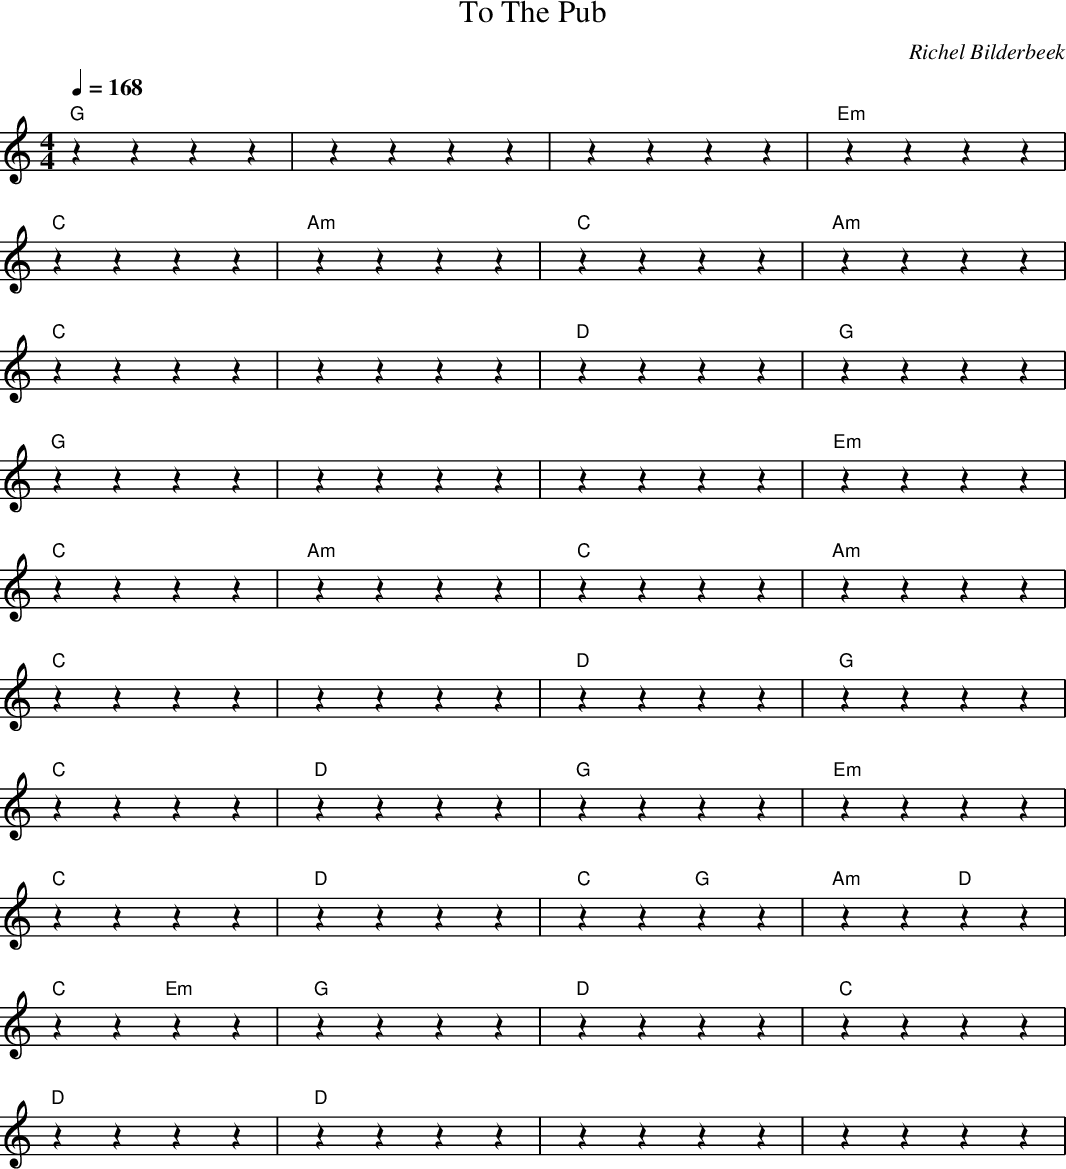
\includegraphics[width=\textwidth,height=\textheight,keepaspectratio]{../songs/42_to_the_pub.png}
%  \caption{To The Pub}
%  \label{fig:42_to_the_pub}
%\end{figure}

%%%%%%%%%%%%%%%%%%%%%%%%%%%%%%%%%%%%%%%%%%%%%%%%%%%%%%%%%%%%%%%%%%%%%%%%%%%%%%%%
\chapter{Even If Your Hair Is Blue}
%%%%%%%%%%%%%%%%%%%%%%%%%%%%%%%%%%%%%%%%%%%%%%%%%%%%%%%%%%%%%%%%%%%%%%%%%%%%%%%%

\lstinputlisting[
  caption = Even If Your Hair Is Blue,
  label = lst:43_even_if_your_hair_is_blue
]{../songs/43_even_if_your_hair_is_blue.txt}

%\begin{figure}[!htbp]
%  \includegraphics[width=\textwidth,height=\textheight,keepaspectratio]{../songs/43_even_if_your_hair_is_blue.png}
%  \caption{Even If Your Hair Is Blue}
%  \label{fig:43_even_if_your_hair_is_blue}
%\end{figure}

%%%%%%%%%%%%%%%%%%%%%%%%%%%%%%%%%%%%%%%%%%%%%%%%%%%%%%%%%%%%%%%%%%%%%%%%%%%%%%%%
\section{Life Is A Bitch}
%%%%%%%%%%%%%%%%%%%%%%%%%%%%%%%%%%%%%%%%%%%%%%%%%%%%%%%%%%%%%%%%%%%%%%%%%%%%%%%%

\lstinputlisting[
  caption = Life Is A Bitch,
  label = lst:44_life_is_a_bitch
]{../songs/44_life_is_a_bitch.txt}

%\begin{figure}[!htbp]
%  \includegraphics[width=\textwidth,height=\textheight,keepaspectratio]{../songs/44_life_is_a_bitch.png}
%  \caption{Life Is A Bitch}
%  \label{fig:44_life_is_a_bitch}
%\end{figure}

%%%%%%%%%%%%%%%%%%%%%%%%%%%%%%%%%%%%%%%%%%%%%%%%%%%%%%%%%%%%%%%%%%%%%%%%%%%%%%%%
\chapter{Plank Op Wieltjes}
%%%%%%%%%%%%%%%%%%%%%%%%%%%%%%%%%%%%%%%%%%%%%%%%%%%%%%%%%%%%%%%%%%%%%%%%%%%%%%%%

\lstinputlisting[
  caption = Plank Op Wieltjes,
  label = lst:45_plank_op_wieltjes
]{../songs/45_plank_op_wieltjes.txt}

%\begin{figure}[!htbp]
%  \includegraphics[width=\textwidth,height=\textheight,keepaspectratio]{../songs/45_plank_op_wieltjes.png}
%  \caption{Plank Op Wieltjes}
%  \label{fig:45_plank_op_wieltjes}
%\end{figure}

%%%%%%%%%%%%%%%%%%%%%%%%%%%%%%%%%%%%%%%%%%%%%%%%%%%%%%%%%%%%%%%%%%%%%%%%%%%%%%%%
\chapter{Koud Bloed In Mijn Hart}
%%%%%%%%%%%%%%%%%%%%%%%%%%%%%%%%%%%%%%%%%%%%%%%%%%%%%%%%%%%%%%%%%%%%%%%%%%%%%%%%

\lstinputlisting[
  caption = Koud Bloed In Mijn Hart,
  label = lst:46_koud_bloed_in_mijn_hart
]{../songs/46_koud_bloed_in_mijn_hart.txt}

\begin{figure}[!htbp]
  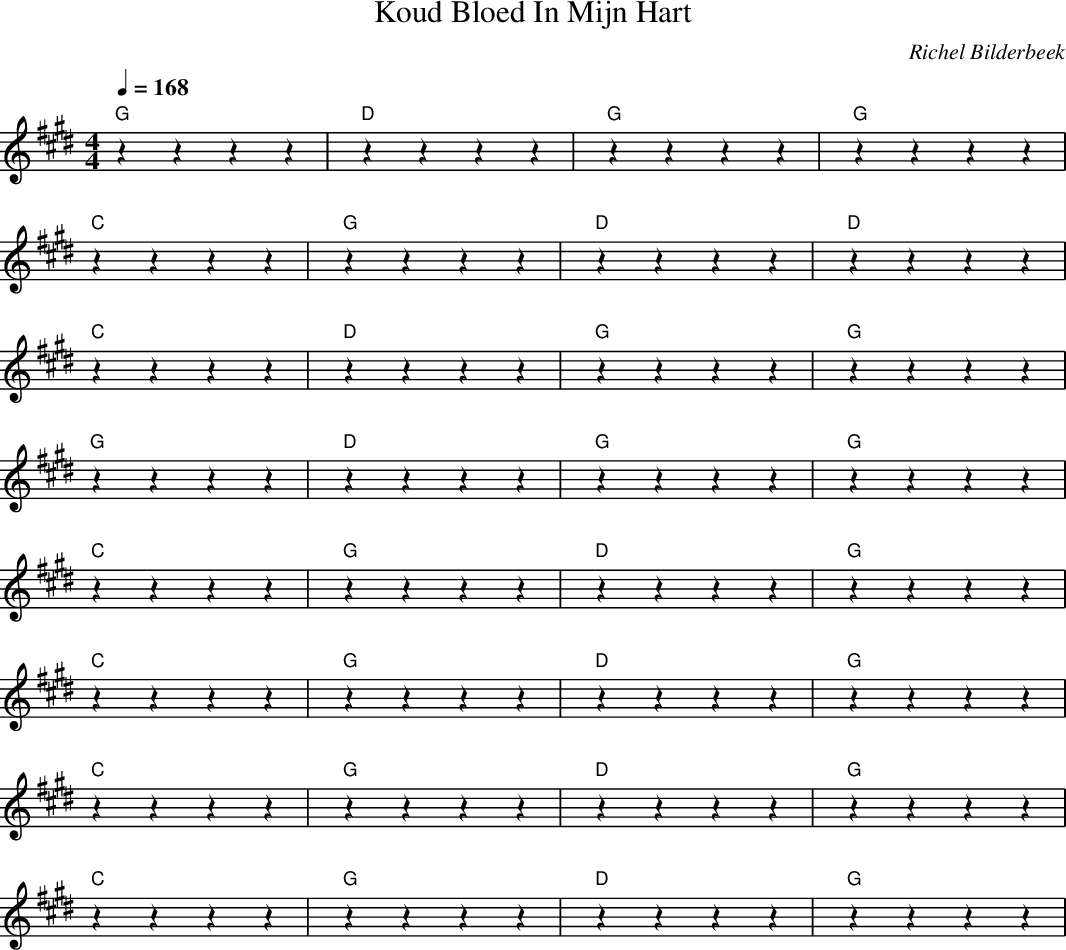
\includegraphics[width=\textwidth,height=\textheight,keepaspectratio]{../songs/46_koud_bloed_in_mijn_hart.png}
  \caption{Koud Bloed In Mijn Hart}
  \label{fig:46_koud_bloed_in_mijn_hart}
\end{figure}

%%%%%%%%%%%%%%%%%%%%%%%%%%%%%%%%%%%%%%%%%%%%%%%%%%%%%%%%%%%%%%%%%%%%%%%%%%%%%%%%
\chapter{Mijn Date Van Vrijdagavond}
%%%%%%%%%%%%%%%%%%%%%%%%%%%%%%%%%%%%%%%%%%%%%%%%%%%%%%%%%%%%%%%%%%%%%%%%%%%%%%%%

\lstinputlisting[
  caption = Mijn Date Van Vrijdagavond,
  label = lst:47_mijn_date_van_vrijdagavond
]{../songs/47_mijn_date_van_vrijdagavond.txt}

%\begin{figure}[!htbp]
%  \includegraphics[width=\textwidth,height=\textheight,keepaspectratio]{../songs/47_mijn_date_van_vrijdagavond.png}
%  \caption{Mijn Date Van Vrijdagavond}
%  \label{fig:47_mijn_date_van_vrijdagavond}
%\end{figure}

%%%%%%%%%%%%%%%%%%%%%%%%%%%%%%%%%%%%%%%%%%%%%%%%%%%%%%%%%%%%%%%%%%%%%%%%%%%%%%%%
\chapter{Achter Mijn Raam}
%%%%%%%%%%%%%%%%%%%%%%%%%%%%%%%%%%%%%%%%%%%%%%%%%%%%%%%%%%%%%%%%%%%%%%%%%%%%%%%%

\lstinputlisting[
  caption = Achter Mijn Raam,
  label = lst:48_achter_mijn_raam
]{../songs/48_achter_mijn_raam.txt}

%\begin{figure}[!htbp]
%  \includegraphics[width=\textwidth,height=\textheight,keepaspectratio]{../songs/48_achter_mijn_raam.png}
%  \caption{Achter Mijn Raam}
%  \label{fig:48_achter_mijn_raam}
%\end{figure}

%%%%%%%%%%%%%%%%%%%%%%%%%%%%%%%%%%%%%%%%%%%%%%%%%%%%%%%%%%%%%%%%%%%%%%%%%%%%%%%%
\section{Ben Ik Een Spin}
%%%%%%%%%%%%%%%%%%%%%%%%%%%%%%%%%%%%%%%%%%%%%%%%%%%%%%%%%%%%%%%%%%%%%%%%%%%%%%%%

\lstinputlisting[
  caption = Ben Ik Een Spin,
  label = lst:49_ben_ik_een_spin
]{../songs/49_ben_ik_een_spin.txt}

%\begin{figure}[!htbp]
%  \includegraphics[width=\textwidth,height=\textheight,keepaspectratio]{../songs/49_ben_ik_een_spin.png}
%  \caption{Ben Ik Een Spin}
%  \label{fig:49_ben_ik_een_spin}
%\end{figure}

%%%%%%%%%%%%%%%%%%%%%%%%%%%%%%%%%%%%%%%%%%%%%%%%%%%%%%%%%%%%%%%%%%%%%%%%%%%%%%%%
\section{Organellenwals}
%%%%%%%%%%%%%%%%%%%%%%%%%%%%%%%%%%%%%%%%%%%%%%%%%%%%%%%%%%%%%%%%%%%%%%%%%%%%%%%%

\lstinputlisting[
  caption = Organellenwals,
  label = lst:50_organellenwals
]{../songs/50_organellenwals.txt}

%\begin{figure}[!htbp]
%  \includegraphics[width=\textwidth,height=\textheight,keepaspectratio]{../songs/50_organellenwals.png}
%  \caption{Organellenwals}
%  \label{fig:50_organellenwals}
%\end{figure}

%%%%%%%%%%%%%%%%%%%%%%%%%%%%%%%%%%%%%%%%%%%%%%%%%%%%%%%%%%%%%%%%%%%%%%%%%%%%%%%%
\section{Stuk Eiwit}
%%%%%%%%%%%%%%%%%%%%%%%%%%%%%%%%%%%%%%%%%%%%%%%%%%%%%%%%%%%%%%%%%%%%%%%%%%%%%%%%

\lstinputlisting[
  caption = Stuk Eiwit,
  label = lst:51_stuk_eiwit
]{../songs/51_stuk_eiwit.txt}

%\begin{figure}[!htbp]
%  \includegraphics[width=\textwidth,height=\textheight,keepaspectratio]{../songs/51_stuk_eiwit.png}
%  \caption{Stuk Eiwit}
%  \label{fig:51_stuk_eiwit}
%\end{figure}

%%%%%%%%%%%%%%%%%%%%%%%%%%%%%%%%%%%%%%%%%%%%%%%%%%%%%%%%%%%%%%%%%%%%%%%%%%%%%%%%
\section{Heejaa Mama}
%%%%%%%%%%%%%%%%%%%%%%%%%%%%%%%%%%%%%%%%%%%%%%%%%%%%%%%%%%%%%%%%%%%%%%%%%%%%%%%%

\lstinputlisting[
  caption = Heejaa Mama,
  label = lst:52_heejaa_mama
]{../songs/52_heejaa_mama.txt}

%\begin{figure}[!htbp]
%  \includegraphics[width=\textwidth,height=\textheight,keepaspectratio]{../songs/52_heejaa_mama.png}
%  \caption{Heejaa Mama}
%  \label{fig:52_heejaa_mama}
%\end{figure}

%%%%%%%%%%%%%%%%%%%%%%%%%%%%%%%%%%%%%%%%%%%%%%%%%%%%%%%%%%%%%%%%%%%%%%%%%%%%%%%%
\section{Voor De Klas}
%%%%%%%%%%%%%%%%%%%%%%%%%%%%%%%%%%%%%%%%%%%%%%%%%%%%%%%%%%%%%%%%%%%%%%%%%%%%%%%%

\lstinputlisting[
  caption = Voor De Klas,
  label = lst:53_voor_de_klas
]{../songs/53_voor_de_klas.txt}

%\begin{figure}[!htbp]
%  \includegraphics[width=\textwidth,height=\textheight,keepaspectratio]{../songs/53_voor_de_klas.png}
%  \caption{Voor De Klas}
%  \label{fig:53_voor_de_klas}
%\end{figure}

%%%%%%%%%%%%%%%%%%%%%%%%%%%%%%%%%%%%%%%%%%%%%%%%%%%%%%%%%%%%%%%%%%%%%%%%%%%%%%%%
\section{Friday}
%%%%%%%%%%%%%%%%%%%%%%%%%%%%%%%%%%%%%%%%%%%%%%%%%%%%%%%%%%%%%%%%%%%%%%%%%%%%%%%%

\lstinputlisting[
  caption = Friday,
  label = lst:54_friday
]{../songs/54_friday.txt}

\begin{figure}[!htbp]
  \includegraphics[width=\textwidth,height=\textheight,keepaspectratio]{../songs/54_friday.png}
  \caption{Friday}
  \label{fig:54_friday}
\end{figure}

%%%%%%%%%%%%%%%%%%%%%%%%%%%%%%%%%%%%%%%%%%%%%%%%%%%%%%%%%%%%%%%%%%%%%%%%%%%%%%%%
\section{Vrouwen Van Je Dromen}
%%%%%%%%%%%%%%%%%%%%%%%%%%%%%%%%%%%%%%%%%%%%%%%%%%%%%%%%%%%%%%%%%%%%%%%%%%%%%%%%

\lstinputlisting[
  caption = Vrouwen Van Je Dromen,
  label = lst:55_vrouwen_van_je_dromen
]{../songs/55_vrouwen_van_je_dromen.txt}

%\begin{figure}[!htbp]
%  \includegraphics[width=\textwidth,height=\textheight,keepaspectratio]{../songs/55_vrouwen_van_je_dromen.png}
%  \caption{Vrouwen Van Je Dromen}
%  \label{fig:55_vrouwen_van_je_dromen}
%\end{figure}

%%%%%%%%%%%%%%%%%%%%%%%%%%%%%%%%%%%%%%%%%%%%%%%%%%%%%%%%%%%%%%%%%%%%%%%%%%%%%%%%
\chapter{Groningen Danst}
%%%%%%%%%%%%%%%%%%%%%%%%%%%%%%%%%%%%%%%%%%%%%%%%%%%%%%%%%%%%%%%%%%%%%%%%%%%%%%%%

\lstinputlisting[
  caption = Groningen Danst,
  label = lst:56_groningen_danst
]{../songs/56_groningen_danst.txt}

%\begin{figure}[!htbp]
%  \includegraphics[width=\textwidth,height=\textheight,keepaspectratio]{../songs/56_groningen_danst.png}
%  \caption{Groningen Danst}
%  \label{fig:56_groningen_danst}
%\end{figure}

%%%%%%%%%%%%%%%%%%%%%%%%%%%%%%%%%%%%%%%%%%%%%%%%%%%%%%%%%%%%%%%%%%%%%%%%%%%%%%%%
\chapter{Superman B}
%%%%%%%%%%%%%%%%%%%%%%%%%%%%%%%%%%%%%%%%%%%%%%%%%%%%%%%%%%%%%%%%%%%%%%%%%%%%%%%%

\lstinputlisting[
  caption = Superman B,
  label = lst:57_superman_b
]{../songs/57_superman_b.txt}

\begin{figure}[!htbp]
  \includegraphics[width=\textwidth,height=\textheight,keepaspectratio]{../songs/57_superman_b.png}
  \caption{Superman B}
  \label{fig:57_superman_b}
\end{figure}

%%%%%%%%%%%%%%%%%%%%%%%%%%%%%%%%%%%%%%%%%%%%%%%%%%%%%%%%%%%%%%%%%%%%%%%%%%%%%%%%
\chapter{Hee Ga Je Mee}
%%%%%%%%%%%%%%%%%%%%%%%%%%%%%%%%%%%%%%%%%%%%%%%%%%%%%%%%%%%%%%%%%%%%%%%%%%%%%%%%

\lstinputlisting[
  caption = Hee Ga Je Mee,
  label = lst:58_hee_ga_je_mee
]{../songs/58_hee_ga_je_mee.txt}

\begin{figure}[!htbp]
  \includegraphics[width=\textwidth,height=\textheight,keepaspectratio]{../songs/58_hee_ga_je_mee.png}
  \caption{Hee Ga Je Mee}
  \label{fig:58_hee_ga_je_mee}
\end{figure}

%%%%%%%%%%%%%%%%%%%%%%%%%%%%%%%%%%%%%%%%%%%%%%%%%%%%%%%%%%%%%%%%%%%%%%%%%%%%%%%%
\section{Een}
%%%%%%%%%%%%%%%%%%%%%%%%%%%%%%%%%%%%%%%%%%%%%%%%%%%%%%%%%%%%%%%%%%%%%%%%%%%%%%%%

\lstinputlisting[
  caption = Een,
  label = lst:59_een
]{../songs/59_een.txt}

%\begin{figure}[!htbp]
%  \includegraphics[width=\textwidth,height=\textheight,keepaspectratio]{../songs/59_een.png}
%  \caption{Een}
%  \label{fig:59_een}
%\end{figure}

%%%%%%%%%%%%%%%%%%%%%%%%%%%%%%%%%%%%%%%%%%%%%%%%%%%%%%%%%%%%%%%%%%%%%%%%%%%%%%%%
\chapter{Liefdeskapitein}
%%%%%%%%%%%%%%%%%%%%%%%%%%%%%%%%%%%%%%%%%%%%%%%%%%%%%%%%%%%%%%%%%%%%%%%%%%%%%%%%

\lstinputlisting[
  caption = Liefdeskapitein,
  label = lst:60_liefdeskapitein
]{../songs/60_liefdeskapitein.txt}

%\begin{figure}[!htbp]
%  \includegraphics[width=\textwidth,height=\textheight,keepaspectratio]{../songs/60_liefdeskapitein.png}
%  \caption{Liefdeskapitein}
%  \label{fig:60_liefdeskapitein}
%\end{figure}

%%%%%%%%%%%%%%%%%%%%%%%%%%%%%%%%%%%%%%%%%%%%%%%%%%%%%%%%%%%%%%%%%%%%%%%%%%%%%%%%
\section{Mars}
%%%%%%%%%%%%%%%%%%%%%%%%%%%%%%%%%%%%%%%%%%%%%%%%%%%%%%%%%%%%%%%%%%%%%%%%%%%%%%%%

\lstinputlisting[
  caption = Mars,
  label = lst:61_mars
]{../songs/61_mars.txt}

%\begin{figure}[!htbp]
%  \includegraphics[width=\textwidth,height=\textheight,keepaspectratio]{../songs/61_mars.png}
%  \caption{Mars}
%  \label{fig:61_mars}
%\end{figure}

%%%%%%%%%%%%%%%%%%%%%%%%%%%%%%%%%%%%%%%%%%%%%%%%%%%%%%%%%%%%%%%%%%%%%%%%%%%%%%%%
\chapter{Pjanoman}
%%%%%%%%%%%%%%%%%%%%%%%%%%%%%%%%%%%%%%%%%%%%%%%%%%%%%%%%%%%%%%%%%%%%%%%%%%%%%%%%

\lstinputlisting[
  caption = Pjanoman,
  label = lst:62_pjanoman
]{../songs/62_pjanoman.txt}

%\begin{figure}[!htbp]
%  \includegraphics[width=\textwidth,height=\textheight,keepaspectratio]{../songs/62_pjanoman.png}
%  \caption{Pjanoman}
%  \label{fig:62_pjanoman}
%\end{figure}

%%%%%%%%%%%%%%%%%%%%%%%%%%%%%%%%%%%%%%%%%%%%%%%%%%%%%%%%%%%%%%%%%%%%%%%%%%%%%%%%
\chapter{Monsieur Pannetier}
%%%%%%%%%%%%%%%%%%%%%%%%%%%%%%%%%%%%%%%%%%%%%%%%%%%%%%%%%%%%%%%%%%%%%%%%%%%%%%%%

\lstinputlisting[
  caption = Monsieur Pannetier,
  label = lst:63_monsieur_pannetier
]{../songs/63_monsieur_pannetier.txt}

%\begin{figure}[!htbp]
%  \includegraphics[width=\textwidth,height=\textheight,keepaspectratio]{../songs/63_monsieur_pannetier.png}
%  \caption{Monsieur Pannetier}
%  \label{fig:63_monsieur_pannetier}
%\end{figure}

%%%%%%%%%%%%%%%%%%%%%%%%%%%%%%%%%%%%%%%%%%%%%%%%%%%%%%%%%%%%%%%%%%%%%%%%%%%%%%%%
\section{16777216 Kleuren}
%%%%%%%%%%%%%%%%%%%%%%%%%%%%%%%%%%%%%%%%%%%%%%%%%%%%%%%%%%%%%%%%%%%%%%%%%%%%%%%%

\lstinputlisting[
  caption = 16777216 Kleuren,
  label = lst:64_16777216_kleuren
]{../songs/64_16777216_kleuren.txt}

%\begin{figure}[!htbp]
%  \includegraphics[width=\textwidth,height=\textheight,keepaspectratio]{../songs/64_16777216_kleuren.png}
%  \caption{16777216 Kleuren}
%  \label{fig:64_16777216_kleuren}
%\end{figure}

%%%%%%%%%%%%%%%%%%%%%%%%%%%%%%%%%%%%%%%%%%%%%%%%%%%%%%%%%%%%%%%%%%%%%%%%%%%%%%%%
\chapter{Dino}
%%%%%%%%%%%%%%%%%%%%%%%%%%%%%%%%%%%%%%%%%%%%%%%%%%%%%%%%%%%%%%%%%%%%%%%%%%%%%%%%

\lstinputlisting[
  caption = Dino,
  label = lst:65_dino
]{../songs/65_dino.txt}

\begin{figure}[!htbp]
  \includegraphics[width=\textwidth,height=\textheight,keepaspectratio]{../songs/65_dino-0.png}
  \caption{Dino 1/2}
  \label{fig:65_dino_1}
\end{figure}

\begin{figure}[!htbp]
  \includegraphics[width=\textwidth,height=\textheight,keepaspectratio]{../songs/65_dino-1.png}
  \caption{Dino 2/2}
  \label{fig:65_dino_2}
\end{figure}

%%%%%%%%%%%%%%%%%%%%%%%%%%%%%%%%%%%%%%%%%%%%%%%%%%%%%%%%%%%%%%%%%%%%%%%%%%%%%%%%
\chapter{Ljum}
%%%%%%%%%%%%%%%%%%%%%%%%%%%%%%%%%%%%%%%%%%%%%%%%%%%%%%%%%%%%%%%%%%%%%%%%%%%%%%%%

\lstinputlisting[
  caption = Ljum,
  label = lst:66_ljum
]{../songs/66_ljum.txt}

%\begin{figure}[!htbp]
%  \includegraphics[width=\textwidth,height=\textheight,keepaspectratio]{../songs/66_ljum.png}
%  \caption{Ljum}
%  \label{fig:66_ljum}
%\end{figure}

%%%%%%%%%%%%%%%%%%%%%%%%%%%%%%%%%%%%%%%%%%%%%%%%%%%%%%%%%%%%%%%%%%%%%%%%%%%%%%%%
\section{Ah! Les Crocodiles}
%%%%%%%%%%%%%%%%%%%%%%%%%%%%%%%%%%%%%%%%%%%%%%%%%%%%%%%%%%%%%%%%%%%%%%%%%%%%%%%%

\lstinputlisting[
  caption = Ah! Les Crocodiles,
  label = lst:xx_ah_les_crocodiles
]{../songs/xx_ah_les_crocodiles.txt}

\begin{figure}[!htbp]
  \includegraphics[width=\textwidth,height=\textheight,keepaspectratio]{../songs/xx_ah_les_crocodiles.png}
  \caption{Ah! Les Crocodiles}
  \label{fig:xx_ah_les_crocodiles}
\end{figure}

%%%%%%%%%%%%%%%%%%%%%%%%%%%%%%%%%%%%%%%%%%%%%%%%%%%%%%%%%%%%%%%%%%%%%%%%%%%%%%%%
\section{Banan}
%%%%%%%%%%%%%%%%%%%%%%%%%%%%%%%%%%%%%%%%%%%%%%%%%%%%%%%%%%%%%%%%%%%%%%%%%%%%%%%%

\lstinputlisting[
  caption = Banan,
  label = lst:xx_banan
]{../songs/xx_banan.txt}

\begin{figure}[!htbp]
  \includegraphics[width=\textwidth,height=\textheight,keepaspectratio]{../songs/xx_banan.png}
  \caption{Banan}
  \label{fig:xx_banan}
\end{figure}

%%%%%%%%%%%%%%%%%%%%%%%%%%%%%%%%%%%%%%%%%%%%%%%%%%%%%%%%%%%%%%%%%%%%%%%%%%%%%%%%
\chapter{Dad}
%%%%%%%%%%%%%%%%%%%%%%%%%%%%%%%%%%%%%%%%%%%%%%%%%%%%%%%%%%%%%%%%%%%%%%%%%%%%%%%%

%\lstinputlisting[
%  caption = Dad,
%  label = lst:xx_dad
%]{../songs/xx_dad.txt}

\begin{figure}[!htbp]
  \includegraphics[width=\textwidth,height=\textheight,keepaspectratio]{../songs/xx_dad-0.png}
  \caption{Dad 1/3}
  \label{fig:xx_dad_1}
\end{figure}

\begin{figure}[!htbp]
  \includegraphics[width=\textwidth,height=\textheight,keepaspectratio]{../songs/xx_dad-1.png}
  \caption{Dad 2/3}
  \label{fig:xx_dad_2}
\end{figure}

\begin{figure}[!htbp]
  \includegraphics[width=\textwidth,height=\textheight,keepaspectratio]{../songs/xx_dad-2.png}
  \caption{Dad 3/3}
  \label{fig:xx_dad_3}
\end{figure}

%%%%%%%%%%%%%%%%%%%%%%%%%%%%%%%%%%%%%%%%%%%%%%%%%%%%%%%%%%%%%%%%%%%%%%%%%%%%%%%%
\chapter{Forever Young}
%%%%%%%%%%%%%%%%%%%%%%%%%%%%%%%%%%%%%%%%%%%%%%%%%%%%%%%%%%%%%%%%%%%%%%%%%%%%%%%%

%\lstinputlisting[
%  caption = Forever Young,
%  label = lst:xx_forever_young
%]{../songs/xx_forever_young.txt}

\begin{figure}[!htbp]
  \includegraphics[width=\textwidth,height=\textheight,keepaspectratio]{../songs/xx_forever_young.png}
  \caption{Forever Young}
  \label{fig:xx_forever_young}
\end{figure}

%%%%%%%%%%%%%%%%%%%%%%%%%%%%%%%%%%%%%%%%%%%%%%%%%%%%%%%%%%%%%%%%%%%%%%%%%%%%%%%%
\section{Moordenaars}
%%%%%%%%%%%%%%%%%%%%%%%%%%%%%%%%%%%%%%%%%%%%%%%%%%%%%%%%%%%%%%%%%%%%%%%%%%%%%%%%

\lstinputlisting[
  caption = Moordenaars,
  label = lst:xx_moordenaars
]{../songs/xx_moordenaars.txt}

%\begin{figure}[!htbp]
%  \includegraphics[width=\textwidth,height=\textheight,keepaspectratio]{../songs/xx_moordenaars.png}
%  \caption{Moordenaars}
%  \label{fig:xx_moordenaars}
%\end{figure}

%%%%%%%%%%%%%%%%%%%%%%%%%%%%%%%%%%%%%%%%%%%%%%%%%%%%%%%%%%%%%%%%%%%%%%%%%%%%%%%%
\chapter{Stars}
%%%%%%%%%%%%%%%%%%%%%%%%%%%%%%%%%%%%%%%%%%%%%%%%%%%%%%%%%%%%%%%%%%%%%%%%%%%%%%%%

\lstinputlisting[
  caption = Stars,
  label = lst:xx_stars
]{../songs/xx_stars.txt}

%\begin{figure}[!htbp]
%  \includegraphics[width=\textwidth,height=\textheight,keepaspectratio]{../songs/xx_stars.png}
%  \caption{Stars}
%  \label{fig:xx_stars}
%\end{figure}

%%%%%%%%%%%%%%%%%%%%%%%%%%%%%%%%%%%%%%%%%%%%%%%%%%%%%%%%%%%%%%%%%%%%%%%%%%%%%%%%
\chapter{Vaar Julskinka Har Rymt}
%%%%%%%%%%%%%%%%%%%%%%%%%%%%%%%%%%%%%%%%%%%%%%%%%%%%%%%%%%%%%%%%%%%%%%%%%%%%%%%%

%\lstinputlisting[
%  caption = Vaar Julskinka Har Rymt,
%  label = lst:xx_vaar_julskinka_har_rymt
%]{../songs/xx_vaar_julskinka_har_rymt.txt}

\begin{figure}[!htbp]
  \includegraphics[width=\textwidth,height=\textheight,keepaspectratio]{../songs/xx_vaar_julskinka_har_rymt-0.png}
  \caption{Vaar Julskinka Har Rymt 1/4}
  \label{fig:xx_vaar_julskinka_har_rymt_1}
\end{figure}

\begin{figure}[!htbp]
  \includegraphics[width=\textwidth,height=\textheight,keepaspectratio]{../songs/xx_vaar_julskinka_har_rymt-1.png}
  \caption{Vaar Julskinka Har Rymt 2/4}
  \label{fig:xx_vaar_julskinka_har_rymt_2}
\end{figure}

\begin{figure}[!htbp]
  \includegraphics[width=\textwidth,height=\textheight,keepaspectratio]{../songs/xx_vaar_julskinka_har_rymt-2.png}
  \caption{Vaar Julskinka Har Rymt 3/4}
  \label{fig:xx_vaar_julskinka_har_rymt_3}
\end{figure}

\begin{figure}[!htbp]
  \includegraphics[width=\textwidth,height=\textheight,keepaspectratio]{../songs/xx_vaar_julskinka_har_rymt-3.png}
  \caption{Vaar Julskinka Har Rymt 4/4}
  \label{fig:xx_vaar_julskinka_har_rymt_4}
\end{figure}

%%%%%%%%%%%%%%%%%%%%%%%%%%%%%%%%%%%%%%%%%%%%%%%%%%%%%%%%%%%%%%%%%%%%%%%%%%%%%%%%
\section{Your Smile}
%%%%%%%%%%%%%%%%%%%%%%%%%%%%%%%%%%%%%%%%%%%%%%%%%%%%%%%%%%%%%%%%%%%%%%%%%%%%%%%%

\lstinputlisting[
  caption = Your Smile,
  label = lst:xx_your_smile
]{../songs/xx_your_smile.txt}

\begin{figure}[!htbp]
  \includegraphics[width=\textwidth,height=\textheight,keepaspectratio]{../songs/xx_your_smile.png}
  \caption{Your Smile}
  \label{fig:xx_your_smile}
\end{figure}


\end{document}
